% !TeX program = xelatex
% !TeX encoding = UTF-8
% Canonical report; frozen physics and saved numerical data.
\documentclass[11pt,a4paper]{article}
\usepackage[left=21mm,right=21mm,top=21mm,bottom=22mm]{geometry}
\usepackage{fontspec}
\setmainfont{Times New Roman}
\usepackage[russian]{babel}
\usepackage{amsmath,amssymb,graphicx,longtable,array}
\setlength{\parindent}{1.2em}
\setlength{\parskip}{.10em}
\setlength{\emergencystretch}{2em}
\linespread{1.03}
\graphicspath{{figures/}}
\newcommand{\dd}{\,\mathrm d}
\newcommand{\trunc}[1]{\left[#1\right]_{\leq3}}
\newcommand{\Gam}{\boldsymbol\Gamma}
\newcommand{\Om}{\boldsymbol\Omega}
\newcommand{\Chi}{\boldsymbol\chi}
\newcommand{\eone}{\mathbf e_1}
\newcommand{\jp}{j_\parallel}
\newcommand{\jb}{j_\perp}
\newcommand{\Bp}{B_\parallel}
\newcommand{\Bb}{B_\perp}
\widowpenalty=10000
\clubpenalty=10000
\begin{document}
\setlength{\abovedisplayskip}{9pt}
\setlength{\belowdisplayskip}{8pt}
\begin{center}
{\Large\bfseries Параметрическая неустойчивость свободных плоских колебаний двух жёстко сопряжённых стержней}\par
\smallskip
Механическая постановка, вывод уравнений и численные результаты\par
{\small Научный отчёт для обсуждения с руководителем\quad 12 октября 2026 г.}
\end{center}

\section{Один стержень: что движется и что деформируется}
\subsection{Ось, сечение и местные направления}
Начнём с одного первоначально прямого стержня. Его ось проходит через центры тяжести поперечных сечений. Материальная координата $s$ отсчитывается вдоль исходной оси; $0\leq s\leq L$. Направление $t$ совпадает с положительным направлением $s$. Впоследствии оба стержня будут ориентированы от внешней заделки к общему узлу.

Поперечное направление $n$ лежит в исходной плоскости конструкции, а $k$ перпендикулярно этой плоскости. Тройка $(t,n,k)$ правая: $t\times n=k$. Толщина $h$ измеряется вдоль $n$, ширина $b$ --- вдоль $k$. Материальные координаты точки сечения обозначим через $\eta$ и $\zeta$ соответственно:
\[
-h/2\leq\eta\leq h/2,\qquad -b/2\leq\zeta\leq b/2.
\]
Это координаты относительно исходного центра тяжести, а не дополнительные неизвестные функции. Схема одного стержня приведена на рис.~\ref{fig:rod}.

\begin{figure}[htbp]
\centering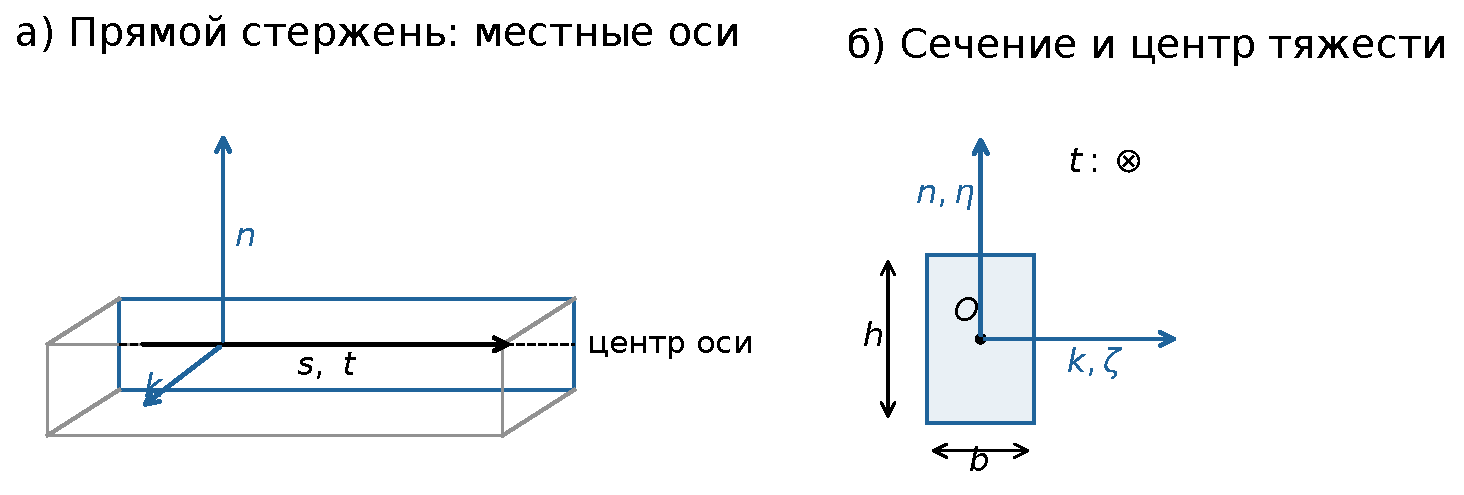
\includegraphics[width=\linewidth]{rod_axes_section.pdf}
\caption{Один прямой стержень и его исходное сечение. Толщина $h$ направлена по $n$, ширина $b$ --- по $k$; $O$ --- центр тяжести. В виде сечения справа $t$ направлен от наблюдателя ($\otimes$). Изометрический вид слева условный; деформация не показана. Локальные направления не следует отождествлять с глобальными осями всей угловой конструкции.}
\label{fig:rod}
\end{figure}

Материал принимается однородным, изотропным и линейно упругим. Геометрия движения может быть нелинейной. Сечение симметрично относительно главных осей. Сохраняются поперечный сдвиг и вращательная инерция; предварительное напряжение, внешняя нагрузка после освобождения и демпфирование отсутствуют.

Ниже используется редуцированная одномерная модель. Она задаёт движение сечения небольшим числом функций вместо полного трёхмерного поля. Такая гипотеза облегчает описание связанных колебаний, но не делает стержневую модель полным следствием трёхмерной упругости.

\subsection{Три перемещения оси и три независимых поворота}
Центр сечения может перемещаться вдоль $t$, $n$ и $k$. Соответствующие поля $u(s,t)$, $w(s,t)$, $v(s,t)$ имеют размерность длины. $u$ описывает продольное перемещение, $w$ --- прогиб в исходной плоскости конструкции, $v$ --- прогиб из неё. Само перемещение сечения ещё не определяет его ориентацию.

Для ориентации вводятся три безразмерные угловые координаты. $\theta$ задаёт положительный поворот вокруг $+k$, $\psi$ --- вокруг $-n$, $\Phi$ --- вокруг $+t$. Положительные направления определяются правилом правого винта. В линейном приближении физический вектор поворота равен
\[
\Phi t-\psi n+\theta k.
\]
Минус перед $\psi$ необходим для принятого соглашения о внеплоскостном сдвиге. При конечных малых поворотах эти три поля являются компонентами вектора экспоненциальных координат с указанным знаком, а не последовательными углами Эйлера.

Рисунок~\ref{fig:motions} отдельно показывает перемещения центра и изменение ориентации сечения. При изгибе ось становится кривой, а поворот каждого сечения остаётся самостоятельной неизвестной. При кручении сечение поворачивается вокруг оси стержня. Изменение угла $\Phi$ вдоль $s$ создаёт крутильную деформацию.

\begin{figure}[htbp]
\centering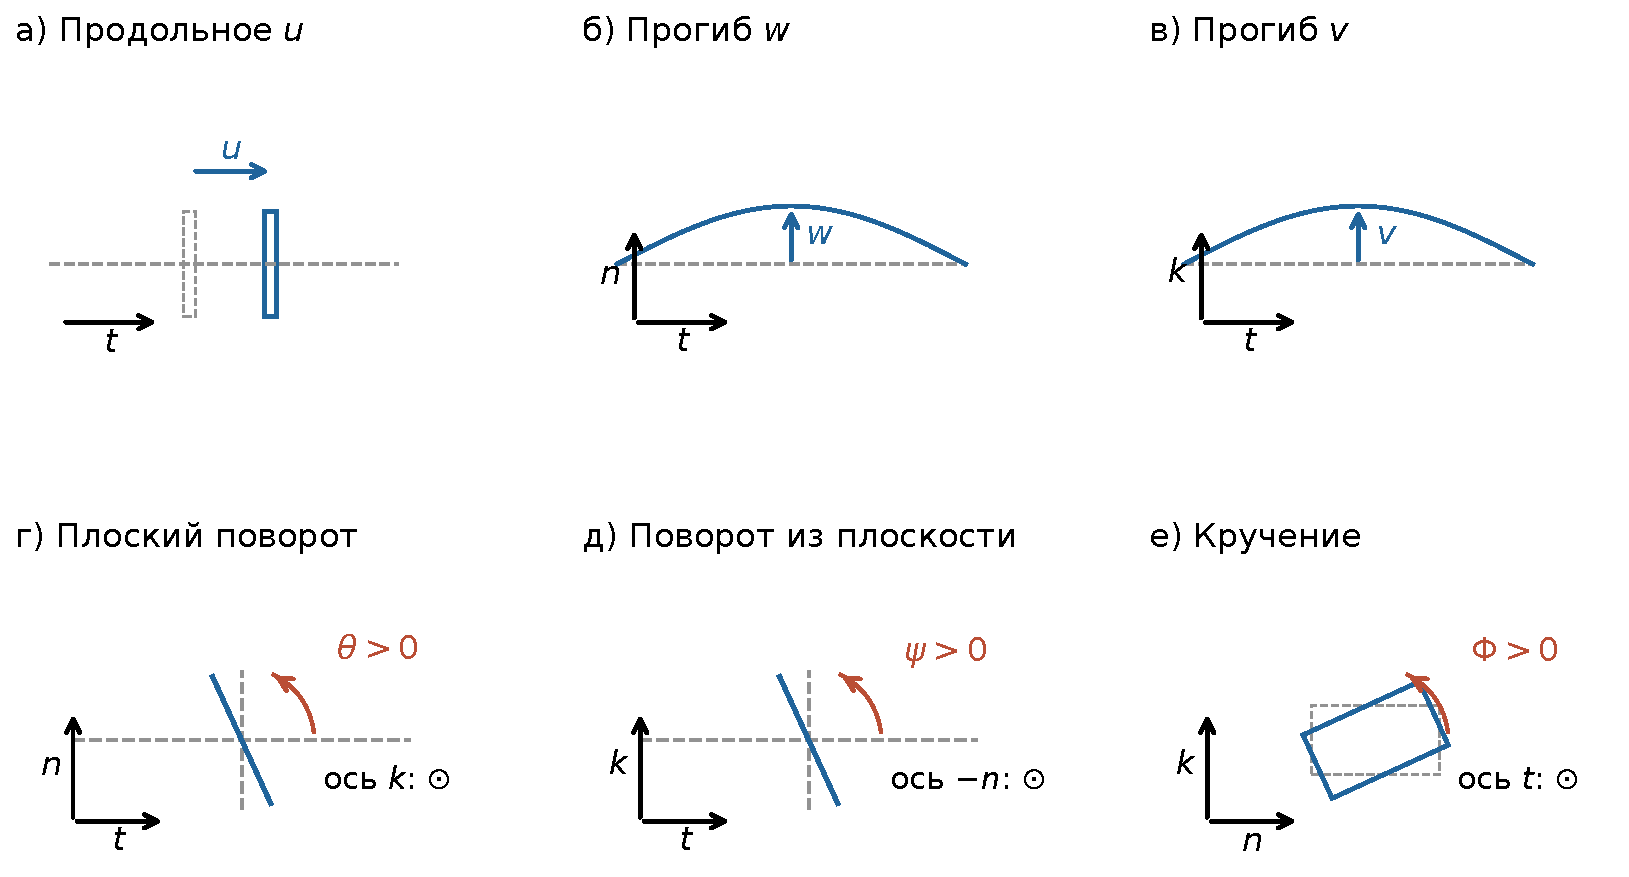
\includegraphics[width=\linewidth]{seven_fields_motion.pdf}
\caption{Шесть движений: а--в) перемещения оси $u,w,v$; г--е) повороты сечения $\theta,\psi,\Phi$. В г) наблюдатель смотрит вдоль $-k$, в д) --- вдоль $+n$, в е) --- вдоль $-t$; обозначенная точкой ось направлена к наблюдателю. Красные стрелки показывают положительные повороты. Пунктир --- исходное положение. Все деформации условно увеличены; кривые а--в не являются рассчитанными собственными формами.}
\label{fig:motions}
\end{figure}

Шести функций недостаточно для выбранного описания продольных колебаний. Необходимо ещё поле, которое характеризует изменение поперечного размера. Оно не перемещает ось и не поворачивает сечение.

\subsection{Седьмая координата: независимая поперечная деформация $c$}
Пусть $d_2,d_3$ --- текущие поперечные направления, поворачивающиеся вместе с сечением, а $\mathbf r$ --- текущий центр. Принято следующее положение материальной точки:
\begin{equation}
\mathbf x(s,\eta,\zeta,t)=\mathbf r(s,t)
+\eta[1+c(s,t)]\mathbf d_2(s,t)+\zeta\mathbf d_3(s,t).
\label{eq:affine}
\end{equation}
Формула~\eqref{eq:affine} сначала переносит центр, затем поворачивает поперечные направления и изменяет масштаб только вдоль $d_2$. Поле $c$ --- безразмерная инженерная поперечная деформация. Разные сечения могут иметь разные значения $c(s,t)$.

Для отдельного сечения из~\eqref{eq:affine} непосредственно следует
\[
h_{\rm new}=h(1+c),\qquad b_{\rm new}=b.
\]
При $c<0$ толщина уменьшается, при $c>0$ увеличивается. На рис.~\ref{fig:contraction} изменение показано в текущих направлениях $d_2,d_3$: поворот этих направлений не меняет смысл $c$.

\begin{figure}[htbp]
\centering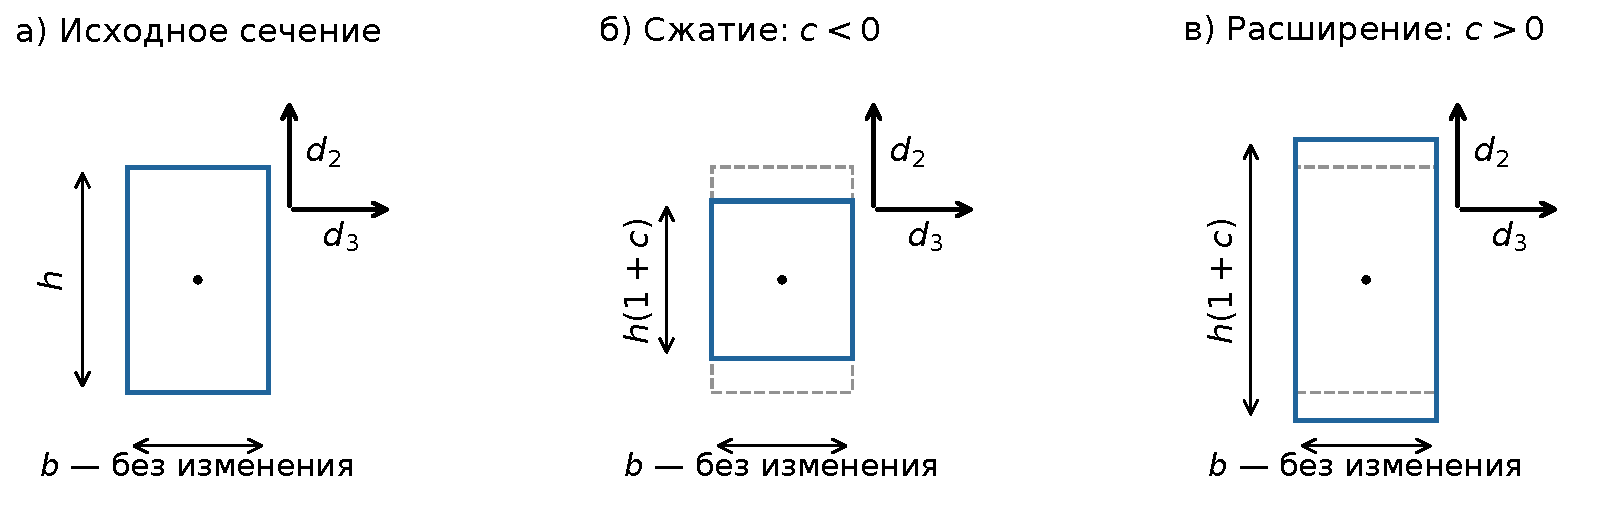
\includegraphics[width=\linewidth]{contraction_section.pdf}
\caption{Изменение одного поперечного размера в принятой кинематике: исходное сечение, сжатие и расширение. Ширина $b$ во всех трёх случаях неизменна. Серый пунктир --- исходный прямоугольник, синяя линия --- текущий. Масштабы изменения условно преувеличены; эта схема не показывает реальную амплитуду рассчитанного $c$.}
\label{fig:contraction}
\end{figure}

Поле $c$ является самостоятельной динамической координатой. Оно не тождественно $-\nu u_s$ и не заменяется этим выражением в полной задаче. Такая связь возникает лишь в определённом низкочастотном пределе.

\textbf{Физическое ограничение.} У свободного изотропного трёхмерного стержня продольное растяжение вызывает пуассоновские деформации в обоих поперечных направлениях. Здесь самостоятельное изменение масштаба описывается только вдоль $d_2$. Отдельного поля изменения ширины нет. Поэтому это не полный трёхмерный учёт эффекта Пуассона; пригодность такой пространственной редукции требует обсуждения.

Таким образом, канонический порядок семи неизвестных имеет вид
\[
q=(u,w,v,\Phi,\psi,\theta,c).
\]
Три поля перемещают ось, три меняют ориентацию сечения, одно меняет его поперечный масштаб. Ни нерастяжимость, ни равенство поворота наклону оси заранее не назначаются.

\section{Линейная кинематика: от движения точки к деформациям}
\subsection{Почему наклон оси не равен повороту сечения}
Если центр соседнего сечения смещается на $w_s\,\dd s$ по $n$, наклон оси в линейном приближении равен $w_s$. Однако поперечное сечение может повернуться на другой угол $\theta$. Отклонение от ортогональности сечения и оси описывает сдвиг
\[
\gamma_{\rm pl}=w_s-\theta.
\]
Аналогично в плоскости $(t,k)$ наклон оси равен $v_s$, а соответствующий поворот --- $\psi$. Поэтому
\[
\gamma_\perp=v_s-\psi.
\]
Рисунок~\ref{fig:shear} показывает эти две независимости. Кинематика Эйлера --- Бернулли потребовала бы нулевого сдвига. В принятой тимошенковской модели этого ограничения нет: сдвиг имеет собственную упругую энергию.

\begin{figure}[htbp]
\centering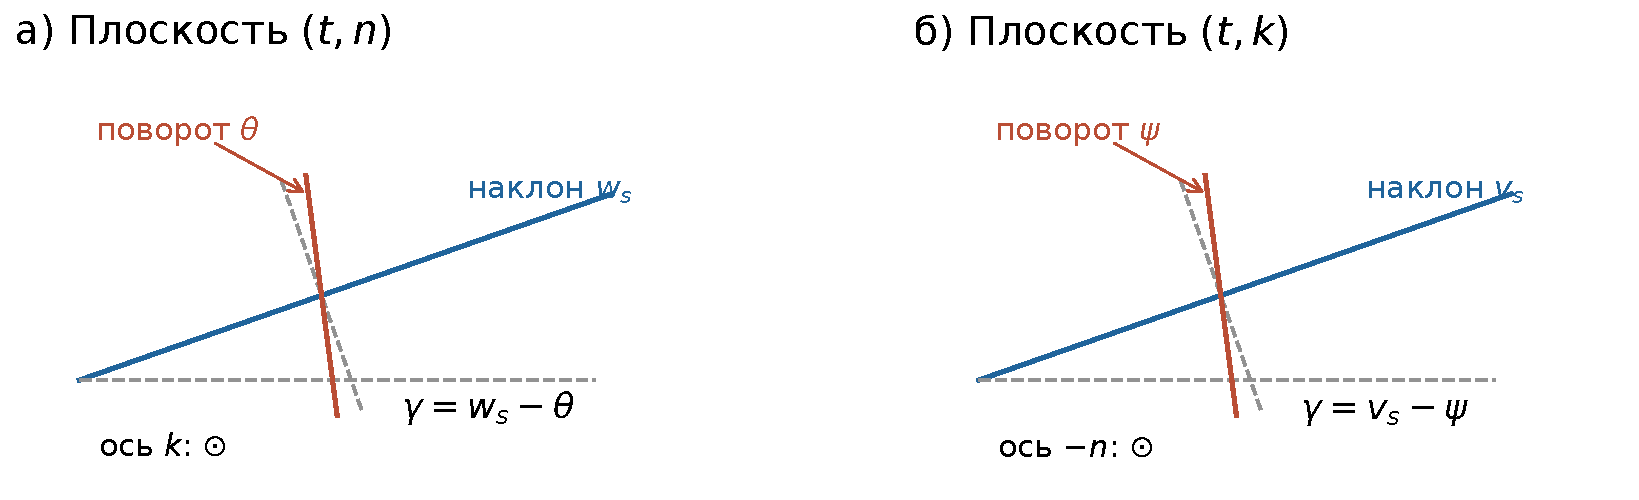
\includegraphics[width=\linewidth]{timoshenko_shear.pdf}
\caption{Наклон оси и поворот сечения: синяя линия --- ось, красная --- независимо повернувшееся сечение, серый наклонный пунктир --- нормаль к текущей оси. Показаны положительные сдвиги $w_s-\theta$ и $v_s-\psi$. Ось положительного поворота направлена к наблюдателю. Углы условно увеличены; отождествление малого угла с производной прогиба относится к линейной кинематике.}
\label{fig:shear}
\end{figure}

\subsection{Объединённое линейное поле материальной точки}
В локальной плоскости $(t,n)$ при малых поворотах принята запись
\begin{equation}
U_x=u-\eta\theta,\qquad U_n=w+\eta c.
\label{eq:linearfield}
\end{equation}
В~\eqref{eq:linearfield} $U_x,U_n$ --- перемещения материальной точки, а $u,w$ --- перемещения центра. Верхняя точка сечения ($\eta>0$) при положительном $\theta$ смещается против $t$, что даёт $-\eta\theta$. Перенос по $n$ равен $w$, дополнительное изменение расстояния от центра --- $\eta c$.

Дифференцирование~\eqref{eq:linearfield} даёт три линейные деформации:
\[
\varepsilon_{xx}=\partial_sU_x=u_s-\eta\theta_s,
\qquad \varepsilon_{nn}=\partial_\eta U_n=c,
\]
\[
\gamma_{xn}=\partial_sU_n+\partial_\eta U_x
=w_s-\theta+\eta c_s.
\]
Часть $u_s$ отвечает за продольное растяжение, $-\eta\theta_s$ --- за неодинаковое растяжение волокон при изгибе. Поле $c$ меняет толщину. Если соседние сечения сжимаются по-разному, возникает дополнительный сдвиг $\eta c_s$. Оставшаяся часть $w_s-\theta$ является тимошенковским сдвигом.

В пространственном линейном пределе той же гипотезы положение точки даёт
\[
U_x=u-\eta\theta+\zeta\psi,\qquad
U_n=w+\eta c-\zeta\Phi,\qquad
U_k=v+\eta\Phi.
\]
Слагаемые с $\Phi$ являются касательными перемещениями при кручении. Знаки $\zeta\psi$ и $-\eta\theta$ следуют из осей положительных поворотов на рис.~\ref{fig:motions}. Эта запись объясняет кинематику; упругий закон ниже принимается отдельно и не выводится произвольным применением одного 3D-закона к сумме всех компонент.

\section{Продольные колебания по Миндлину --- Геррманну}
\subsection{Физическая идея и литературное основание}
При растяжении стержень обычно сужается поперёк. В элементарной продольной теории это изменение либо не имеет своей динамики, либо исключается квазистатически. Идея модели Миндлина --- Геррманна состоит в сохранении независимой поперечной деформации, её инерции и неоднородности вдоль стержня.

Здесь используется вариант редуцированного сочетания M--H и Тимошенко по Jang, Park, Lee~\cite{jang}. В работе Rucka~\cite{rucka} такое сочетание применено к стержневой угловой конструкции. Исходная работа Миндлина --- Геррманна известна по вторичной ссылке [35] у Rucka; её полный текст непосредственно не использовался.

Из Jang заимствуется линейное редуцированное основание без композитной накладки. Нелинейное продолжение, используемое далее, является принятой проектной моделью и не приписывается этим авторам. Поправочные коэффициенты M--H различаются между источниками. Поэтому параметры Rucka, подобранные для её волнового эксперимента, не заменяют принятые здесь коэффициенты.

\subsection{Два конститутивных вклада и интегрирование по сечению}
В продольном M--H-вкладе сохраняются две нормальные деформации $u_s,c$. При исключении напряжений в направлении ширины принят редуцированный закон
\[
\sigma_{xx}=\frac{E}{1-\nu^2}(u_s+\nu c),\qquad
\sigma_{nn}=\frac{E}{1-\nu^2}(c+\nu u_s).
\]
Связь Пуассона отражается в перекрёстных членах. В отдельном изгибном вкладе дополнительно исключается поперечное нормальное напряжение, поэтому нормальный изгибный модуль равен $E$. Сумма этих двух выбранных вкладов соответствует принятой редукции Jang. Она не равносильна использованию одного неизменённого трёхмерного закона для полного объединённого поля.

В продольном блоке плотность нормальной энергии равна
\[
\tfrac12(\sigma_{xx}u_s+\sigma_{nn}c)
=\frac{E}{2(1-\nu^2)}(u_s^2+2\nu u_sc+c^2).
\]
К этой энергии добавляется сдвиговый вклад $\kappa G(\eta c_s)^2/2$. Здесь $G=E/[2(1+\nu)]$ --- модуль сдвига, а $\kappa=5/6$ --- принятое проектное значение поправочного коэффициента. Его численное значение не заявляется как установленное авторами Jang.

Интегрируем по исходному прямоугольнику. Для центрированного сечения
\[
\int_{A_0}\dd A=A_0=bh,\qquad
\int_{A_0}\eta\dd A=0,\qquad
\int_{A_0}\eta^2\dd A=I_\parallel=\frac{bh^3}{12}.
\]
Нормальная энергия умножается на площадь, энергия $c_s$ --- на момент площади. Поэтому
\[
C=\frac{EA_0}{1-\nu^2},\qquad H=\kappa G I_\parallel.
\]
$C$ --- нормальная жёсткость выбранного закона. $H$ характеризует сопротивление неоднородной поперечной деформации: даже при одинаковом среднем сжатии распределения $c(s)$ с большим градиентом имеют дополнительную энергию.

Продольная скорость точки равна $u_t$, а поперечная скорость от изменения толщины --- $\eta c_t$. Интегрирование суммы их квадратов по исходной массе даёт
\[
\int_{A_0}\frac{\rho}{2}(u_t^2+\eta^2c_t^2)\dd A
=\frac12(mu_t^2+j_\parallel c_t^2),
\quad m=\rho A_0,\quad j_\parallel=\rho I_\parallel.
\]
$m$ есть масса единицы длины. $j_\parallel$ здесь является инерционным коэффициентом изменения толщины; позднее тот же момент массы определяет инерцию плоского поворота.

В итоге энергии одного стержня равны
\begin{equation}
\begin{aligned}
V_{\rm MH}&=\frac12\int_0^L
\bigl[C(u_s^2+2\nu u_sc+c^2)+Hc_s^2\bigr]\dd s,\\
T_{\rm MH}&=\frac12\int_0^L
\bigl[mu_t^2+j_\parallel c_t^2\bigr]\dd s.
\end{aligned}
\label{eq:MHenergy}
\end{equation}
Все подынтегральные величины в~\eqref{eq:MHenergy} имеют размерность энергии на единицу длины. Введение $c$ сохраняет и нормальную связь, и градиентную жёсткость, и отдельную инерцию.

\subsection{Вариация: от энергии к двум уравнениям}
Рассмотрим действие $\int(T_{\rm MH}-V_{\rm MH})\dd t$. Вариации $\delta u,\delta c$ равны нулю в начальный и конечный моменты, но внутри интервала независимы. Сначала дифференцируем потенциальную энергию:
\[
\delta V_{\rm MH}=\int_0^L
\{C(u_s+\nu c)\delta u_s+C(c+\nu u_s)\delta c
+Hc_s\delta c_s\}\dd s.
\]
Обозначим продольную силу $N=C(u_s+\nu c)$ и усилие, сопряжённое градиенту $c$, через $R_c=Hc_s$. Интегрирование по частям переносит производные с вариаций на усилия:
\[
\delta V_{\rm MH}=[N\delta u+R_c\delta c]_0^L
+\int_0^L\{-N_s\delta u+[C(c+\nu u_s)-(R_c)_s]\delta c\}\dd s.
\]
Граничные члены одновременно определяют механические концевые усилия. Нормальная сила сопряжена $u$, а $R_c$ --- независимому изменению толщины.

Для кинетической энергии интегрирование по времени даёт
\[
\delta\int T_{\rm MH}\dd t
=-\int\!\int_0^L(mu_{tt}\delta u+j_\parallel c_{tt}\delta c)\dd s\dd t.
\]
Теперь коэффициенты при двух произвольных вариациях в действии должны исчезнуть. Получаем
\begin{equation}
\boxed{\begin{aligned}
mu_{tt}&=[C(u_s+\nu c)]_s,\\
j_\parallel c_{tt}&=(Hc_s)_s-C(c+\nu u_s).
\end{aligned}}
\label{eq:MH}
\end{equation}
В первом уравнении~\eqref{eq:MH} ускорение оси определяется разностью продольных сил на соседних сечениях. Во втором инерция изменения толщины уравновешивается градиентным усилием и нормальным восстанавливающим вкладом. Член $-\nu C u_s$ связывает продольное растяжение с поперечным сужением.

\subsection{Связь с обычным продольным стержнем}
Если инерционный вклад $j_\parallel c_{tt}$ и градиентный вклад $(Hc_s)_s$ малы относительно нормальных членов, второе уравнение~\eqref{eq:MH} даёт
\[
c\approx-\nu u_s.
\]
Тогда продольная сила становится
\[
N\approx C(1-\nu^2)u_s=EA_0u_s.
\]
Так восстанавливается классическая продольная жёсткость $EA_0$. Самостоятельная координата $c$ не противоречит обычной теории: последняя получается при её квазистатическом исключении. Однако это приближение не действует автоматически на всех частотах и у заделок, где задано независимое условие на $c$.

\section{Два изгиба и кручение: энергии и вариационный вывод}
\subsection{Плоский изгиб Тимошенко}
Пусть сначала действуют только $w$ и $\theta$. Волокно на расстоянии $\eta$ от центра растягивается на $-\eta\theta_s$. В принятом изгибном конститутивном вкладе его энергия равна $E\eta^2\theta_s^2/2$. Интегрирование по сечению даёт жёсткость $B_\parallel=EI_\parallel$. Сдвиг $w_s-\theta$ имеет жёсткость $S=\kappa GA_0$.

Точка сечения движется по $n$ со скоростью $w_t$ и вдоль оси со скоростью $-\eta\theta_t$. Следовательно,
\[
\begin{aligned}
V_{\rm pl}&=\frac12\int_0^L[S(w_s-\theta)^2+B_\parallel\theta_s^2]\dd s,\\
T_{\rm pl}&=\frac12\int_0^L[mw_t^2+j_\parallel\theta_t^2]\dd s.
\end{aligned}
\]
Кривизна в линейном приближении равна $\theta_s$, а не $w_{ss}$: последняя совпала бы с ней только при дополнительном бессдвиговом ограничении.

Введём поперечную силу $Q=S(w_s-\theta)$ и изгибающий момент $M=B_\parallel\theta_s$. Вариация потенциала равна
\[
\begin{aligned}
\delta V_{\rm pl}
&=\int_0^L[Q\delta w_s-Q\delta\theta+M\delta\theta_s]\dd s\\
&=[Q\delta w+M\delta\theta]_0^L
+\int_0^L[-Q_s\delta w-(Q+M_s)\delta\theta]\dd s.
\end{aligned}
\]
Вариация кинетической энергии в действии даёт $-mw_{tt}\delta w-j_\parallel\theta_{tt}\delta\theta$. Независимость $\delta w,\delta\theta$ приводит к
\[
mw_{tt}=Q_s,\qquad j_\parallel\theta_{tt}=M_s+Q.
\]
Первый баланс описывает поступательное движение, второй --- вращение сечения. Знак $+Q$ во втором уравнении следует из слагаемого $-Q\delta\theta$ в потенциальной энергии. Поэтому знак момента сдвиговой силы согласован с определением $w_s-\theta$, а не выбирается отдельно.

\subsection{Изгиб из плоскости}
Теперь рассматриваются $v$ и $\psi$. Положительный $\psi$ направлен вокруг $-n$, поэтому продольное перемещение точки при этом повороте равно $+\zeta\psi$. Нормальная изгибная деформация равна $\zeta\psi_s$, сдвиг --- $v_s-\psi$.

Интеграл квадрата координаты по ширине даёт другой момент площади:
\[
I_\perp=\int_{A_0}\zeta^2\dd A=\frac{hb^3}{12},\qquad
B_\perp=EI_\perp,\qquad j_\perp=\rho I_\perp.
\]
Даже при изотропном материале изгибные жёсткости различаются вследствие геометрии. Если $h>b$, то $I_\parallel>I_\perp$: сечение сильнее сопротивляется изгибу в плоскости $(t,n)$. Изотропия относится к свойствам материала, а не к форме сечения.

Энергии внеплоскостного изгиба имеют вид
\[
\begin{aligned}
V_\perp&=\frac12\int_0^L[S(v_s-\psi)^2+B_\perp\psi_s^2]\dd s,\\
T_\perp&=\frac12\int_0^L[mv_t^2+j_\perp\psi_t^2]\dd s.
\end{aligned}
\]
Положим $Q_\perp=S(v_s-\psi)$, $M_\perp=B_\perp\psi_s$. По тем же двум интегрированиям по частям получаем
\[
\delta V_\perp=[Q_\perp\delta v+M_\perp\delta\psi]_0^L
+\int_0^L[-(Q_\perp)_s\delta v-((M_\perp)_s+Q_\perp)\delta\psi]\dd s.
\]
Отсюда следуют балансы $mv_{tt}=(Q_\perp)_s$ и $j_\perp\psi_{tt}=(M_\perp)_s+Q_\perp$. Их структура совпадает с плоским изгибом, но момент площади и ось положительного поворота другие.

\subsection{Кручение}
При изменении $\Phi$ вдоль оси соседние сечения поворачиваются на разные углы. Крутильная кривизна в линейном приближении равна $\Phi_s$. Для принятой обобщённой редукции сечения~\cite{yartsev} обозначим её жёсткость через $C_T$. Она учитывает принятую конденсацию депланации; самостоятельная динамическая координата депланации здесь не вводится.

Скорости точки от кручения равны $-\zeta\Phi_t$ по $n$ и $\eta\Phi_t$ по $k$. Их квадраты дают полярный момент \emph{массы} $j_\parallel+j_\perp$. Энергии равны
\[
V_T=\frac12\int_0^L C_T\Phi_s^2\dd s,\qquad
T_T=\frac12\int_0^L(j_\parallel+j_\perp)\Phi_t^2\dd s.
\]
Для крутящего момента $M_T=C_T\Phi_s$ вариация потенциала равна
\[
\delta V_T=[M_T\delta\Phi]_0^L-\int_0^L(M_T)_s\delta\Phi\dd s.
\]
Поэтому $(j_\parallel+j_\perp)\Phi_{tt}=(C_T\Phi_s)_s$. Упругая крутильная жёсткость не равна автоматически $G(I_\parallel+I_\perp)$: полярный момент, определяющий инерцию, и эффективная жёсткость прямоугольника --- разные величины. Действующее определение $C_T$ приведено в приложении.

\subsection{Все семь линейных уравнений в одном месте}
Соберём полученные балансы в каноническом порядке полей:
\begin{equation}
\boxed{\begin{aligned}
mu_{tt}&=[C(u_s+\nu c)]_s,\\
mw_{tt}&=[S(w_s-\theta)]_s,\\
mv_{tt}&=[S(v_s-\psi)]_s,\\
(j_\parallel+j_\perp)\Phi_{tt}&=(C_T\Phi_s)_s,\\
j_\perp\psi_{tt}&=(B_\perp\psi_s)_s+S(v_s-\psi),\\
j_\parallel\theta_{tt}&=(B_\parallel\theta_s)_s+S(w_s-\theta),\\
j_\parallel c_{tt}&=(Hc_s)_s-C(c+\nu u_s).
\end{aligned}}
\label{eq:linear7}
\end{equation}
Система~\eqref{eq:linear7} содержит три поступательных, три вращательных баланса и баланс изменения толщины. В каждой левой части стоит соответствующая инерция. В первых трёх правых частях --- градиент силы; в трёх вращательных --- градиент момента и, при изгибе, момент сдвиговой силы. Последнее уравнение описывает градиентное сопротивление и нормальную связь Пуассона.

Внутри одного прямого плеча линейные блоки $(u,c)$, $(w,\theta)$, $(v,\psi)$ и $\Phi$ разделены. Это свойство принятой редуцированной энергии и симметричного центрированного сечения. В угловой конструкции общие узловые перемещения и повороты связывают локальные компоненты разных плеч.

\section{Физические коэффициенты и размерности}
Ниже приведены все коэффициенты, входящие в линейные энергии и сохраняемые в нелинейном продолжении. Размерности записаны в SI для пояснения физического смысла. В численном исследовании использованы нормированные единицы, поэтому $E=\rho=1$ не определяет реальный материал и физическую секунду.

\begin{longtable}{>{\raggedright\arraybackslash}p{.09\linewidth}>{\raggedright\arraybackslash}p{.24\linewidth}>{\raggedright\arraybackslash}p{.13\linewidth}>{\raggedright\arraybackslash}p{.43\linewidth}}
\caption{Материал, геометрия, жёсткости и инерционные коэффициенты.}\label{tab:coeff}\\
\hline
Символ & Формула / определение & Размерность & Смысл и место в уравнениях\\\hline
\endfirsthead
\hline Символ & Формула / определение & Размерность & Смысл и место в уравнениях\\\hline
\endhead
$E$ & Модуль Юнга & Н/м$^2$ & Нормальная упругость; определяет $C$, $B_\parallel$, $B_\perp$.\\[5pt]
$\rho$ & Плотность & кг/м$^3$ & Определяет массу и все инерционные коэффициенты.\\[5pt]
$\nu$ & Коэффициент Пуассона & 1 & Связывает $u_s$ и $c$ в нормальном блоке.\\[5pt]
$G$ & $E/[2(1+\nu)]$ & Н/м$^2$ & Модуль сдвига; входит в $S,H,C_T$.\\[5pt]
$\kappa$ & $5/6$ & 1 & Принятая поправка к двум редуцированным сдвиговым энергиям.\\[5pt]
$A_0$ & $bh$ & м$^2$ & Исходная площадь; входит в продольную и сдвиговую жёсткости, массу.\\[5pt]
$I_\parallel$ & $bh^3/12$ & м$^4$ & $\int\eta^2\dd A$; плоский изгиб и изменение толщины.\\[5pt]
$I_\perp$ & $hb^3/12$ & м$^4$ & $\int\zeta^2\dd A$; внеплоскостный изгиб.\\[5pt]
$m$ & $\rho A_0$ & кг/м & Масса единицы длины; уравнения $u,w,v$.\\[5pt]
$j_\parallel$ & $\rho I_\parallel$ & кг$\cdot$м & Инерция $\theta,c$ и часть крутильной инерции.\\[5pt]
$j_\perp$ & $\rho I_\perp$ & кг$\cdot$м & Инерция $\psi$ и часть крутильной инерции.\\[5pt]
$C$ & $EA_0/(1-\nu^2)$ & Н & Нормальная жёсткость M--H; усилия в $u,c$.\\[5pt]
$H$ & $\kappa G I_\parallel$ & Н$\cdot$м$^2$ & Градиентная жёсткость поля $c$; $(Hc_s)_s$.\\[5pt]
$S$ & $\kappa GA_0$ & Н & Сдвиговая жёсткость; силы при двух изгибах.\\[5pt]
$B_\parallel$ & $EI_\parallel$ & Н$\cdot$м$^2$ & Жёсткость плоского изгиба; момент при $\theta_s$.\\[5pt]
$B_\perp$ & $EI_\perp$ & Н$\cdot$м$^2$ & Жёсткость внеплоскостного изгиба; момент при $\psi_s$.\\[5pt]
$C_T$ & Прямоугольный ряд~\eqref{eq:CT} & Н$\cdot$м$^2$ & Крутящий момент при $\Phi_s$; формула в приложении.\\\hline
\end{longtable}

Таблица~\ref{tab:coeff} отделяет жёсткости от инерции. Например, $Hc_s$ имеет размерность Н$\cdot$м и сопряжено безразмерному $c$, тогда как $S(w_s-\theta)$ имеет размерность силы. Повороты $\Phi,\psi,\theta$ и $c$ безразмерны; кривизны имеют размерность м$^{-1}$.

Далее жирным символом $\boldsymbol\Omega$ обозначается трёхкомпонентная угловая скорость сечения, с размерностью времени$^{-1}$. Скаляр $\Omega$ обозначает угловую частоту периодического движения всей конструкции. Эти величины имеют одинаковую размерность, но разный физический смысл.

\section{Зачем нужна нелинейная геометрия и как она вводится}
\subsection{Конечное основное движение и малое возмущение}
Линейная система определяет собственные частоты и формы около недеформированного состояния. Её коэффициенты не зависят от текущей амплитуды колебаний. Поэтому она не описывает изменение уравнений малого внеплоскостного возмущения под действием конечного плоского движения.

Для этой задачи сохраняются нелинейные геометрические и инерционные связи. Например, поперечное движение меняет продольную деформацию оси; сила в повёрнутом сечении меняет направление; изменение толщины меняет вращательную инерцию. Это взаимодействия самой конструкции, а не дополнительно приложенная пространственная сила.

\subsection{Поворот сечения и компоненты деформации}
Положение оси сначала задаётся физическими перемещениями:
\[
\mathbf r=\mathbf r_0+u t+w n+v k.
\]
Следовательно, касательный вектор оси имеет исходные локальные компоненты $(1+u_s,w_s,v_s)$. Чтобы измерить деформацию относительно повернувшегося сечения, этот вектор нужно выразить в текущих направлениях. Поэтому конечные меры имеют скалярный смысл
\[
1+\Gamma_1=\mathbf d_1\cdot\mathbf r_s,\qquad
\Gamma_2=\mathbf d_2\cdot\mathbf r_s,\qquad
\Gamma_3=\mathbf d_3\cdot\mathbf r_s.
\]
$\Gamma_1$ --- продольная деформация относительно направления сечения, $\Gamma_2,\Gamma_3$ --- два сдвига. Они не зависят от общего жёсткого переноса или поворота конструкции.

Для компактного вычисления введём $B=[t,n,k]$, $\mathbf U=(u,w,v)^T$ и вектор поворота $\mathbf a=(\Phi,-\psi,\theta)^T$. Матрица
\[
R=\exp([\mathbf a]_\times),\qquad [\mathbf a]_\times\mathbf b=\mathbf a\times\mathbf b
\]
поворачивает исходные локальные направления; столбцы $BR$ равны $\mathbf d_1,\mathbf d_2,\mathbf d_3$. Это геометрический оператор ориентации, а не новое материальное свойство. В этих обозначениях
\begin{equation}
\Gam=R^T(\eone+\mathbf U_s)-\eone,
\qquad [\Chi]_\times=R^TR_s,
\qquad [\Om]_\times=R^TR_t.
\label{eq:measures}
\end{equation}
В~\eqref{eq:measures} $\chi_1$ --- крутильная кривизна, $\chi_2,\chi_3$ --- изгибные кривизны вокруг текущих поперечных направлений. $\Omega_1,\Omega_2,\Omega_3$ --- компоненты угловой скорости в текущем локальном базисе.

Чтобы увидеть связи без матричных операторов, раскроем деформации по амплитуде. Верхний индекс $[r]$ означает однородную степень $r$ по полям и их производным. Линейные части равны
\[
\Gamma_1^{[1]}=u_s,\qquad
\Gamma_2^{[1]}=w_s-\theta,\qquad
\Gamma_3^{[1]}=v_s-\psi.
\]
Квадратичные поправки имеют вид
\begin{equation}
\begin{aligned}
\Gamma_1^{[2]}&=\theta w_s+\psi v_s-\tfrac12(\theta^2+\psi^2),\\
\Gamma_2^{[2]}&=-\theta u_s+\Phi v_s-\tfrac12\Phi\psi,\\
\Gamma_3^{[2]}&=-\psi u_s-\Phi w_s+\tfrac12\Phi\theta.
\end{aligned}
\label{eq:Gamma2}
\end{equation}
Слагаемые~\eqref{eq:Gamma2} показывают конкретное происхождение связи движений. Продольная деформация содержит произведения прогиба и поворота. Если только для интерпретации взять бессдвиговое приближение $\theta\approx w_s$, $\psi\approx v_s$, её квадратичная часть становится $(w_s^2+v_s^2)/2$. Это знакомое геометрическое растяжение оси; данные равенства не накладываются на нашу систему.

Внеплоскостный сдвиг получает член $-\Phi w_s$: закручивание меняет направление сечения относительно уже искривлённой плоской оси. Обратная связь $+\Phi v_s$ появляется в плоском сдвиге. Знаки в этих двух членах определяются выбранными осями и знаком $-\psi$.

Аналогично первые две степени кривизн равны
\[
\begin{aligned}
\chi_1&=\Phi_s+\tfrac12(\psi\theta_s-\theta\psi_s)+O(\varepsilon_a^3),\\
\chi_2&=-\psi_s+\tfrac12(\Phi\theta_s-\theta\Phi_s)+O(\varepsilon_a^3),\\
\chi_3&=\theta_s+\tfrac12(\Phi\psi_s-\psi\Phi_s)+O(\varepsilon_a^3).
\end{aligned}
\]
Угловые скорости получаются заменой индекса $s$ на $t$ в этих рядах. Например, $\Omega_1=\Phi_t+(\psi\theta_t-\theta\psi_t)/2+O(\varepsilon_a^3)$. Поэтому именованные угловые скорости полей не тождественны компонентам физической угловой скорости при конечном повороте.

\subsection{Потенциальная энергия: каждый механизм отдельно}
Нелинейный упругий закон выбирается так, чтобы сохранять проверенный линейный предел и объективные меры. Его скалярные вклады на единицу исходной длины равны
\[
\begin{aligned}
V_{\rm normal}^{(0)}&=\tfrac C2\Gamma_1^2+\nu Cc\Gamma_1+\tfrac C2c^2,\\
V_{\rm gradient}^{(0)}&=\tfrac H2c_s^2,\\
V_{\rm shear}^{(0)}&=\tfrac S2\Gamma_2^2+\tfrac S2\Gamma_3^2,\\
V_{\rm bend}^{(0)}&=\tfrac{B_\perp}{2}\chi_2^2+\tfrac{B_\parallel}{2}\chi_3^2,\\
V_{\rm twist}^{(0)}&=\tfrac{C_T}{2}\chi_1^2.
\end{aligned}
\]
Первый вклад объединяет продольную и поперечную нормальные деформации. Его положительность и классический предел видны из равенства
\[
V_{\rm normal}^{(0)}=\frac{EA_0}{2}\Gamma_1^2
+\frac C2(c+\nu\Gamma_1)^2.
\]
Градиентный вклад сопротивляется различию толщин соседних сечений; остальные вклады отвечают двум сдвигам, двум изгибам и кручению.

Сумму удобно записать в векторном виде после определения всех скалярных частей:
\begin{equation}
\begin{aligned}
V^{(0)}&=\tfrac12\Gam^TD_\Gamma\Gam+\nu Cc\Gamma_1
+\tfrac C2c^2+\tfrac H2c_s^2+\tfrac12\Chi^TD_\chi\Chi,\\
D_\Gamma&=\operatorname{diag}(C,S,S),\qquad
D_\chi=\operatorname{diag}(C_T,B_\perp,B_\parallel).
\end{aligned}
\label{eq:V0}
\end{equation}
Плотность~\eqref{eq:V0} является \emph{принятым нелинейным продолжением} редуцированной стержневой модели. Она не является единственным полным выводом из трёхмерного закона Гука. В частности, коэффициенты вычисляются по исходному сечению и не меняются с $c$. Дополнительные упругие члены $c\chi_3^2$, $c\Gamma_2^2$ не включены как конститутивное допущение, хотя они не обязаны иметь более высокий амплитудный порядок.

\subsection{Кинетическая энергия и изменение вращательной инерции}
В отличие от упругого закона, инерция непосредственно определяется скоростями аффинного поля~\eqref{eq:affine} и исходной массой. Пусть $\dot{\mathbf d}_j=\boldsymbol\omega_{\rm spatial}\times\mathbf d_j$. Скорость точки равна
\[
\mathbf x_t=\mathbf r_t+\eta c_t\mathbf d_2
+\eta(1+c)\dot{\mathbf d}_2+\zeta\dot{\mathbf d}_3.
\]
При интегрировании квадрата скорости исчезают члены с $\int\eta\dd A$, $\int\zeta\dd A$, $\int\eta\zeta\dd A$, поскольку ось проходит через центр тяжести, а сечение симметрично. Член с $c_t$ ортогонален скорости вращения направления $d_2$. Остаётся скалярная плотность
\begin{equation}
\begin{aligned}
T^{(0)}={}&\tfrac m2(u_t^2+w_t^2+v_t^2)+\tfrac{j_\parallel}{2}c_t^2\\
&+\tfrac12[j_\perp+(1+c)^2j_\parallel]\Omega_1^2
+\tfrac{j_\perp}{2}\Omega_2^2
+\tfrac{(1+c)^2j_\parallel}{2}\Omega_3^2.
\end{aligned}
\label{eq:T0}
\end{equation}
Плотность~\eqref{eq:T0} имеет прозрачный геометрический смысл. При кручении вокруг $d_1$ изменяется расстояние точек по толщине, но не по ширине. При вращении вокруг $d_3$ все расстояния по толщине умножаются на $1+c$. Вращение вокруг $d_2$ определяется неизменным размером по ширине.

Поэтому в компактной записи вращательная часть равна $\Om^TJ(c)\Om/2$, где
\[
J(c)=\operatorname{diag}\bigl(j_\perp+(1+c)^2j_\parallel,\ j_\perp,\ (1+c)^2j_\parallel\bigr).
\]
Общая масса не меняется: интегрирование выполнено по исходным материальным точкам. Множитель $1+c$ перед всей кинетической энергией не вводится. Постоянные упругие жёсткости и меняющееся распределение инерции являются двумя отдельно принятыми элементами редукции; их сочетание не заявляется как полный учёт изменения сечения в 3D-упругости.

\subsection{Конкретные смешанные члены и амплитудное усечение}
Подстановка~\eqref{eq:Gamma2} в нормальную энергию даёт, среди других кубических членов,
\[
+\nu Cc\,\psi v_s-\tfrac12\nu Cc\,\psi^2,
\qquad +C u_s\psi v_s-\tfrac12C u_s\psi^2.
\]
На фоне заданных $c,u_s$ эти члены меняют квадратичную энергию внеплоскостного возмущения. Сдвиговый вклад также содержит $S\Phi\psi w_s/2-S\Phi\theta v_s/2$. В кинетической энергии имеются $j_\parallel c\Phi_t^2$ и $j_\parallel c\theta_t^2$. Они показывают упругие и инерционные пути взаимодействия; один отдельно выписанный член ещё не определяет знак роста.

Исходное редуцированное действие строится из $T^{(0)}-V^{(0)}$. Однако непосредственно решаемая система получается из его амплитудного полинома. Все семь полей и нормированные производные считаются величинами одного малого порядка $\varepsilon_a$; коэффициенты и длины фиксированы. Тогда
\[
T=T_2+T_3+T_4+\cdots,\qquad
V=V_2+V_3+V_4+\cdots.
\]
Нижний индекс здесь означает однородную амплитудную степень. При вариации число множителей поля уменьшается на один, поэтому действие четвёртой степени даёт уравнения третьей степени:
\begin{equation}
\mathcal S_{\leq4}=\int\!\int_0^L
\bigl(T_2+T_3+T_4-V_2-V_3-V_4\bigr)\dd s\dd t,
\qquad E_q^{[1]}+E_q^{[2]}+E_q^{[3]}=0.
\label{eq:quartic}
\end{equation}
В~\eqref{eq:quartic} $u$ и $c$ заранее не понижаются до второго порядка. Сохраняются произведения первого и третьего порядков, а не только квадраты второго. В приложении приведены точные ряды, которые полностью определяют действие и его кубические уравнения.

Малость деформаций и возможность конечного поворота в геометрической записи различаются. Неусечённые меры объективны при жёстком движении. Их кубическое координатное разложение предназначено для малых, но конечных амплитуд, а не для произвольно больших углов. Вариационный подход к пространственным стержням представлен, например, в~\cite{crespo}; авторская бессдвиговая кинематика и иное упорядочение амплитуд сюда не переносились.

\section{Семь нелинейных балансов и решаемые координатные уравнения}
\subsection{Скалярные силы, моменты и импульсы}
Из производных скалярных энергий вводятся усилия в текущем локальном базисе:
\[
N_1=C(\Gamma_1+\nu c),\qquad N_2=S\Gamma_2,\qquad N_3=S\Gamma_3,
\]
\[
M_1=C_T\chi_1,\qquad M_2=B_\perp\chi_2,\qquad M_3=B_\parallel\chi_3.
\]
$N_1$ --- продольная сила; $N_2,N_3$ --- силы сдвига. $M_1$ --- крутящий момент, $M_2,M_3$ --- изгибающие моменты вокруг $d_2,d_3$. В частности, в линейном пределе $M_2=-B_\perp\psi_s$, поскольку положительный $\psi$ направлен вокруг $-n$.

Компоненты вращательного импульса равны
\[
\ell_1=[j_\perp+(1+c)^2j_\parallel]\Omega_1,
\qquad \ell_2=j_\perp\Omega_2,
\qquad \ell_3=(1+c)^2j_\parallel\Omega_3.
\]
Эти компоненты выражены в повёрнутом базисе. Переход к инерциальному балансу поэтому даёт не только $\partial_t\ell_i$, но и члены вращения самого базиса.

\subsection{Основные шаги вариации пространственного действия}
При изменении оси на $\delta\mathbf U$ вариация деформации равна $R^T\delta\mathbf U_s$. Её работа в потенциале составляет
\[
\mathbf N\cdot R^T\delta\mathbf U_s
=(R\mathbf N)\cdot\delta\mathbf U_s.
\]
Интегрирование по $s$ даёт граничную силу $R\mathbf N$ и объёмный член $-\partial_s(R\mathbf N)$. Вариация поступательной кинетической энергии после интегрирования по $t$ даёт $-m\mathbf U_{tt}$. Так возникают три поступательных баланса.

Для поворота сечения допустимая малая вариация записывается $\delta R=R[\boldsymbol\xi]_\times$. Вектор $\boldsymbol\xi$ обозначает малый физический поворот в текущем базисе. Если $\mathbf g=(1+\Gamma_1,\Gamma_2,\Gamma_3)^T$, то
\[
\delta\Gam\big|_{\rm rotation}=-\boldsymbol\xi\times\mathbf g,
\qquad \delta\Chi=\boldsymbol\xi_s+\Chi\times\boldsymbol\xi,
\qquad \delta\Om=\boldsymbol\xi_t+\Om\times\boldsymbol\xi.
\]
Поэтому в вариации потенциала появляются $\mathbf M\cdot\boldsymbol\xi_s$ и
$-(\mathbf g\times\mathbf N+\Chi\times\mathbf M)\cdot\boldsymbol\xi$.
В вариации вращательной кинетической энергии ---
$\boldsymbol\ell\cdot\boldsymbol\xi_t-(\Om\times\boldsymbol\ell)\cdot\boldsymbol\xi$.
После переноса производных с $\boldsymbol\xi$ получаются градиент момента и гироскопические члены. Каждый перекрёстный член ниже таким образом имеет определённый источник в виртуальной работе.

Вариация по $c$ отличается от поворота. Упругий нормальный вклад равен $C(c+\nu\Gamma_1)\delta c$, градиентный --- $Hc_s\delta c_s$. Из кинетической энергии добавляется $j_\parallel(1+c)(\Omega_1^2+\Omega_3^2)\delta c$. Его знак в уравнении определяется разностью $T-V$.

\subsection{Семь неусечённых скалярных балансов}
Пусть $R_{ij}$ --- компоненты матрицы поворота. Три баланса перемещений оси имеют вид
\begin{equation}
\begin{aligned}
mu_{tt}&=\partial_s(R_{11}N_1+R_{12}N_2+R_{13}N_3),\\
mw_{tt}&=\partial_s(R_{21}N_1+R_{22}N_2+R_{23}N_3),\\
mv_{tt}&=\partial_s(R_{31}N_1+R_{32}N_2+R_{33}N_3).
\end{aligned}
\label{eq:transfull}
\end{equation}
В~\eqref{eq:transfull} внутренние силы сначала поворачиваются в исходные локальные направления, затем берётся их градиент. Это объясняет, почему продольная сила может участвовать в поперечном балансе на искривлённой оси.

Обозначим левые части трёх материальных вращательных балансов через $\mathcal B_1,\mathcal B_2,\mathcal B_3$:
\begin{equation}
\begin{aligned}
\mathcal B_1={}&\partial_t\ell_1+\Omega_2\ell_3-\Omega_3\ell_2
-\partial_sM_1-\chi_2M_3+\chi_3M_2
-\Gamma_2N_3+\Gamma_3N_2=0,\\
\mathcal B_2={}&\partial_t\ell_2+\Omega_3\ell_1-\Omega_1\ell_3
-\partial_sM_2-\chi_3M_1+\chi_1M_3\\
&-\Gamma_3N_1+(1+\Gamma_1)N_3=0,\\
\mathcal B_3={}&\partial_t\ell_3+\Omega_1\ell_2-\Omega_2\ell_1
-\partial_sM_3-\chi_1M_2+\chi_2M_1\\
&-(1+\Gamma_1)N_2+\Gamma_2N_1=0.
\end{aligned}
\label{eq:rotfull}
\end{equation}
В~\eqref{eq:rotfull} первая группа --- изменение углового импульса в инерциальном пространстве, вторая --- градиент и перенос внутренних моментов, последняя --- момент внутренних сил. Эти три уравнения сначала записаны вокруг материальных направлений $d_1,d_2,d_3$, а не непосредственно по координатам $\Phi,\psi,\theta$.

Седьмой баланс равен
\begin{equation}
j_\parallel c_{tt}=(Hc_s)_s-C(c+\nu\Gamma_1)
+j_\parallel(1+c)(\Omega_1^2+\Omega_3^2).
\label{eq:cfull}
\end{equation}
Последний член~\eqref{eq:cfull} следует из зависимости инерции от толщины. Он сохраняется даже при $\nu=0$; поэтому отсутствие связи Пуассона само по себе не позволяет удалить $c$ из вращательной динамики.

Формулы~\eqref{eq:transfull}--\eqref{eq:cfull} --- семь балансов \emph{неусечённых принятых редуцированных энергий}. Они полезны для понимания механики. В научных расчётах использовано их согласованное кубическое координатное разложение, которое теперь зададим отдельно.

\subsection{Почему вращательные балансы преобразуются к координатам}
При конечном повороте $\boldsymbol\xi$ не равен $(\delta\Phi,-\delta\psi,\delta\theta)^T$. Связь определяется правым Jacobian экспоненциальных координат:
\[
\boldsymbol\xi=J_r(\mathbf a)P\delta\mathbf z,\qquad
\mathbf z=(\Phi,\psi,\theta)^T,\quad P=\operatorname{diag}(1,-1,1),
\]
\[
J_r(\mathbf a)=I-\tfrac12[\mathbf a]_\times+\tfrac16[\mathbf a]_\times^2+\cdots.
\]
Равенство виртуальных работ
$\boldsymbol{\mathcal B}\cdot\boldsymbol\xi
=(P^TJ_r^T\boldsymbol{\mathcal B})\cdot\delta\mathbf z$
определяет именно транспонированный переход. Поэтому координатный вращательный остаток равен $P^TJ_r^T\boldsymbol{\mathcal B}$. Нельзя просто назвать $\mathcal B_2$ уравнением для $\psi$: уже линейно имеется минус, а нелинейно --- смешивание трёх компонент.

\subsection{Все семь фактически решаемых кубических уравнений}
Для любого выражения $F$ обозначим через $[F]_{\leq3}$ ряд после умножения всех полей и их производных на $\varepsilon_a$, с сохранением степеней 1--3. Усечение выполняется \emph{после} перехода к именованным углам.

Поступательные уравнения и уравнение $c$ имеют скалярную форму
\begin{equation}
\boxed{\begin{aligned}
mu_{tt}&=\partial_s\trunc{R_{11}N_1+R_{12}N_2+R_{13}N_3},\\
mw_{tt}&=\partial_s\trunc{R_{21}N_1+R_{22}N_2+R_{23}N_3},\\
mv_{tt}&=\partial_s\trunc{R_{31}N_1+R_{32}N_2+R_{33}N_3},\\
j_\parallel c_{tt}&=(Hc_s)_s-C(c+\nu[\Gamma_1]_{\leq3})
+\trunc{j_\parallel(1+c)(\Omega_1^2+\Omega_3^2)}.
\end{aligned}}
\label{eq:cubictrans}
\end{equation}
Остальные три уравнения раскрывают тот же переход $J_r^T$ покомпонентно. Положим $a^2=\Phi^2+\psi^2+\theta^2$ и
$d=\Phi\mathcal B_1-\psi\mathcal B_2+\theta\mathcal B_3$; здесь $d$ --- лишь скалярное сокращение, не поперечное направление. Тогда
\begin{equation}
\boxed{\begin{aligned}
0=E_\Phi={}&\trunc{\mathcal B_1
-\tfrac12(\psi\mathcal B_3+\theta\mathcal B_2)
+\tfrac16(\Phi d-a^2\mathcal B_1)},\\
0=E_\psi={}&-\trunc{\mathcal B_2
+\tfrac12(\theta\mathcal B_1-\Phi\mathcal B_3)
+\tfrac16(-\psi d-a^2\mathcal B_2)},\\
0=E_\theta={}&\trunc{\mathcal B_3
+\tfrac12(\Phi\mathcal B_2+\psi\mathcal B_1)
+\tfrac16(\theta d-a^2\mathcal B_3)}.
\end{aligned}}
\label{eq:cubicrot}
\end{equation}
В~\eqref{eq:cubicrot} $\mathcal B_i$ определены скалярными выражениями~\eqref{eq:rotfull}. В произведениях с одним углом нужны степени $\mathcal B_i$ до 2, а в произведениях с двумя углами --- только степень 1. Это прямо следует из общей операции $[\cdot]_{\leq3}$.

Системы~\eqref{eq:cubictrans},~\eqref{eq:cubicrot} содержат все семь \emph{координатных} уравнений принятого действия~\eqref{eq:quartic}. Для восстановления каждого коэффициента достаточно скалярных $N_i,M_i,\ell_i$, компонент $R$, рядов $\Gamma_i,\chi_i,\Omega_i$ и указанного усечения. Их полные необходимые степени определены в приложении. Таким образом, вычислительная система не заменена только абстрактным условием стационарности действия.

Коэффициенты при ускорениях зависят от состояния. После дискретизации получается переменная симметричная матрица масс и нелинейные инерционные члены. Численный переход к первому порядку обращает эту принятую матрицу; уравнения не заменяются двумя искусственными осцилляторами с подогнанной кубической жёсткостью.

\subsection{Что связывает три внеплоскостных поля с плоским движением}
Линейная часть внеплоскостных уравнений есть строки для $v,\Phi,\psi$ в~\eqref{eq:linear7}. Для наглядности из сохранённого полиномиального раскрытия приведём полную квадратичную часть поступательного остатка $E_v$:
\[
E_v^{[2]}=\partial_s\left\{\tfrac S2\Phi\theta
-\psi\bigl[\nu Cc+(C-S)u_s\bigr]\right\}.
\]
На плоском фоне $u_s,c,\theta$ становятся заданными функциями времени и координаты. Поэтому уже эта часть меняет линейный оператор по $\psi,\Phi$.

Квадратичная часть $E_\Phi$ содержит, в частности,
\[
2j_\parallel(c\Phi_{tt}+c_t\Phi_t)
+\tfrac S2(\psi w_s-\theta v_s)
+\tfrac{B_\parallel-C_T}{2}\psi\theta_{ss}
+\tfrac{C_T-B_\perp}{2}\theta\psi_{ss}.
\]
Здесь видны переменная крутильная инерция и смешанные изгибно-крутильные усилия. Это выбранные члены, а не полная квадратичная строка. Аналогично $E_\psi^{[2]}$ содержит
\[
\nu Cc(v_s-\psi)+(C-S)u_s v_s+(2S-C)u_s\psi
+\tfrac S2\Phi w_s.
\]
Оставшиеся инерционные, градиентные и кубические члены сохраняются в~\eqref{eq:cubictrans},~\eqref{eq:cubicrot}; они не отбрасываются в анализе устойчивости. Эти примеры объясняют механизм связи, но не заменяют полный аналитический Jacobian системы.

\section{Явная плоская система: четыре кубических уравнения}
\subsection{Геометрия и неусечённая запись}
При строго плоском движении $v=\Phi=\psi=0$. Остаются $u,w,\theta,c$. Сечение поворачивается только вокруг $k$. Проецирование касательного вектора оси на повернувшиеся направления даёт
\[
\Gamma_1=(1+u_s)\cos\theta+w_s\sin\theta-1,
\qquad
\Gamma_2=-(1+u_s)\sin\theta+w_s\cos\theta.
\]
Положим $N=C(\Gamma_1+\nu c)$, $Q=S\Gamma_2$. Сила $(N,Q)$ повёрнута относительно исходной оси на $\theta$. Поэтому её исходные продольная и поперечная компоненты равны $N\cos\theta-Q\sin\theta$ и $N\sin\theta+Q\cos\theta$.

Четыре неусечённых уравнения принятой редуцированной модели имеют вид
\begin{equation}
\begin{aligned}
mu_{tt}&=(N\cos\theta-Q\sin\theta)_s,\\
mw_{tt}&=(N\sin\theta+Q\cos\theta)_s,\\
\partial_t[j_\parallel(1+c)^2\theta_t]
&=(B_\parallel\theta_s)_s+(1+\Gamma_1)Q-\Gamma_2N,\\
j_\parallel c_{tt}&=(Hc_s)_s-C(c+\nu\Gamma_1)
+j_\parallel(1+c)\theta_t^2.
\end{aligned}
\label{eq:planarfull}
\end{equation}
В~\eqref{eq:planarfull} первые два уравнения учитывают изменение направления внутренних сил. В третьем изменение углового импульса связано с изгибающим моментом и моментом сил $Q,N$. В четвёртом вращение влияет на толщину через инерцию. Эта тригонометрическая форма объясняет геометрию, но непосредственно в расчётах используется её кубическое разложение.

\subsection{Раскрытие геометрии и сил до третьей степени}
Вводя $\sin\theta=\theta-\theta^3/6+\cdots$ и $\cos\theta=1-\theta^2/2+\cdots$, получаем
\[
\begin{aligned}
\relax[\Gamma_1]_{\leq3}&=u_s+\theta w_s-\tfrac12\theta^2-\tfrac12u_s\theta^2,\\
[\Gamma_2]_{\leq3}&=w_s-\theta-u_s\theta-\tfrac12w_s\theta^2+\tfrac16\theta^3.
\end{aligned}
\]
Здесь $\theta w_s-\theta^2/2$ --- ведущая геометрическая поправка к растяжению, $-u_s\theta$ --- изменение сдвига при продольной деформации. Следующие члены необходимы, поскольку энергия сохраняется до четвёртой степени.

Обозначим через $F_u,F_w$ кубически усечённые компоненты силы по исходным $t,n$. В результате согласованного перемножения рядов они равны
\begin{equation}
\begin{aligned}
F_u={}&C(u_s+\nu c)
+(C-S)\theta w_s+(S-\tfrac C2)\theta^2\\
&+(S-C)u_s\theta^2-\tfrac{C\nu}{2}c\theta^2,\\
F_w={}&S(w_s-\theta)+(C-S)u_s\theta+C\nu c\theta\\
&+(C-S)w_s\theta^2+(\tfrac{2S}{3}-\tfrac C2)\theta^3.
\end{aligned}
\label{eq:planarforces}
\end{equation}
В~\eqref{eq:planarforces} первые строки начинаются с линейных сил. Последующие члены происходят одновременно из нелинейной деформации и поворота сил; один из этих двух источников нельзя исключить при сохранении другого.

Для момента внутренних сил в уравнении $\theta$ введём скаляр $\mathcal Q_\theta$. Его полное раскрытие до степени 3 равно
\begin{equation}
\begin{aligned}
\mathcal Q_\theta={}&S(w_s-\theta)
+(S-C)u_s w_s+(C-2S)u_s\theta-C\nu c(w_s-\theta)\\
&+(C-S)u_s^2\theta+(S-C)\theta w_s^2
+(\tfrac{3C}{2}-2S)\theta^2w_s\\
&+(\tfrac{2S}{3}-\tfrac C2)\theta^3+C\nu c u_s\theta.
\end{aligned}
\label{eq:planartorque}
\end{equation}
Формула~\eqref{eq:planartorque} является раскрытием $[(1+\Gamma_1)Q-\Gamma_2N]_{\leq3}$. Поэтому это не новый эмпирический изгибный закон: все коэффициенты уже определены исходной энергией.

\subsection{Полная плоская кубическая система и смысл её членов}
Используя~\eqref{eq:planarforces},~\eqref{eq:planartorque}, получаем четыре реально решаемых плоских уравнения:
\begin{equation}
\boxed{\begin{aligned}
mu_{tt}&=(F_u)_s,\\
mw_{tt}&=(F_w)_s,\\
j_\parallel\bigl[(1+2c+c^2)\theta_{tt}
+2(1+c)c_t\theta_t\bigr]
&=B_\parallel\theta_{ss}+\mathcal Q_\theta,\\
j_\parallel c_{tt}&=Hc_{ss}-C(c+\nu u_s)
-C\nu\theta w_s+\tfrac{C\nu}{2}\theta^2\\
&\quad+\tfrac{C\nu}{2}u_s\theta^2
+j_\parallel\theta_t^2+j_\parallel c\theta_t^2.
\end{aligned}}
\label{eq:planarcubic}
\end{equation}
В~\eqref{eq:planarcubic} все силы и моменты раскрыты выше, поэтому четыре уравнения можно восстановить без обращения к внешнему полиномиальному перечню. При неоднородных коэффициентах внутри плеча следует сохранить дивергентную запись $(B_\parallel\theta_s)_s$, $(Hc_s)_s$; здесь каждый стержень однороден.

В уравнении $u$ члены с $\theta w_s,\theta^2$ описывают растяжение из-за изгиба. В уравнении $w$ члены с $u_s\theta,c\theta$ показывают влияние нормальной силы на поперечный баланс. Кубические произведения уточняют эти связи в принятом амплитудном порядке.

Слева в уравнении $\theta$ стоит производная переменного вращательного импульса. Множитель $1+2c+c^2$ меняет инерцию, а $2(1+c)c_t\theta_t$ отражает её изменение во времени. В уравнении $c$ первые нормальные члены совпадают с M--H, геометрические поправки содержат изгиб, а $j_\parallel(1+c)\theta_t^2$ возникает из вращательной кинетической энергии.

Идеальное плоское движение остаётся плоским из-за зеркальной симметрии. Отражение относительно исходной плоскости меняет знаки $v,\Phi,\psi$, оставляя $u,w,\theta,c$ неизменными. Принятое действие инвариантно при таком отражении. Поэтому при нулевых пространственных полях и скоростях соответствующие три уравнения имеют нулевой остаток. Это утверждение об инвариантности, а не об устойчивости к малому отклонению.

\section{Два стержня: геометрия, заделки и условия в узле}
\subsection{От местной кинематики к общей конструкции}
Теперь соединяем два описанных стержня. Внешние концы неподвижно закреплены. Внутренние концы совпадают в идеальном жёстком точечном узле без массы и эксцентриситета. Жёсткость соединения означает общие перемещение узла и изменение пространственной ориентации при сохранении исходного угла между плечами.

На рис.~\ref{fig:geometry} введены глобальные оси $E_X,E_Y,E_Z$. Они служат для сопоставления разных локальных направлений, а не заменяют координаты $s_i$.
\begin{figure}[htbp]
\centering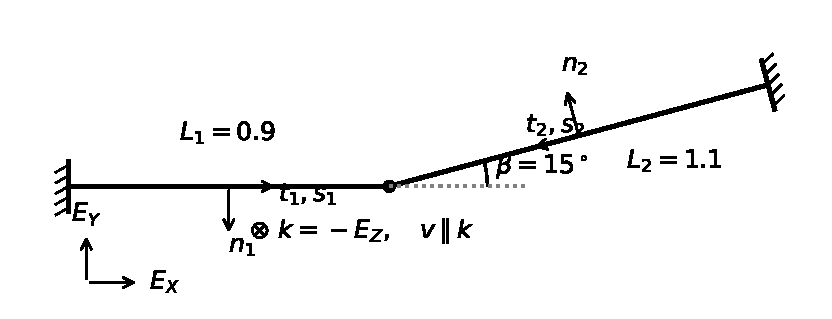
\includegraphics[width=.94\linewidth]{supervisor_geometry.pdf}
\caption{Исходная угловая конструкция и принятые направления. Положительные $s_i$ идут от заделок к узлу, $k=-E_Z$. Угол $\beta$ измеряется между $+E_X$ и лучом от узла к правой заделке; $\beta=0$ означает прямую конструкцию. Показаны реальные пропорции исследованной геометрии; деформации отсутствуют.}
\label{fig:geometry}
\end{figure}

Для обоих плеч сохраняется правый локальный базис $B_i=[t_i,n_i,k]$. Его направления равны
\[
\begin{aligned}
t_1&=E_X,& n_1&=-E_Y,& k&=-E_Z,\\
t_2&=(-\cos\beta,-\sin\beta,0)^T,&
n_2&=(-\sin\beta,\cos\beta,0)^T.
\end{aligned}
\]
При $\beta=0$ материальные координаты направлены навстречу друг другу. Угол $15^\circ$ здесь не является внутренним острым углом между двумя лучами плеч; это отклонение от прямолинейной конфигурации.

\subsection{Заделки и совместность в узле}
На внешнем конце $s_i=0$ задаются семь условий
\[
u_i=w_i=v_i=\Phi_i=\psi_i=\theta_i=c_i=0.
\]
Ось не перемещается, сечение не поворачивается, его независимая поперечная координата закреплена. Дополнительные условия на $w_{i,s}$ или $v_{i,s}$ не назначаются: это было бы несогласованным ограничением сдвиговой кинематики.

В узле $s_i=L_i$ равенство глобальных перемещений означает покомпонентно
\[
\sum_{\alpha=1}^3(B_1)_{j\alpha}(U_1)_\alpha
=\sum_{\alpha=1}^3(B_2)_{j\alpha}(U_2)_\alpha,
\qquad j=X,Y,Z.
\]
Одна и та же локальная координата $u_i$ может иметь разные глобальные направления. Например, продольное перемещение правого плеча имеет одновременно компоненты по $E_X$ и $E_Y$.

Общие координаты узла удобно обозначить через $\mathbf d_J$ (перемещение), $\boldsymbol\alpha_J$ (вектор приращения поворота) и $c_J$. Совместность записывается
\begin{equation}
B_i\mathbf U_i(L_i)=\mathbf d_J,\qquad
B_iP\mathbf z_i(L_i)=\boldsymbol\alpha_J,\qquad
c_i(L_i)=c_J,\quad i=1,2.
\label{eq:compat}
\end{equation}
В общей малой области экспоненциальных координат второе условие~\eqref{eq:compat} эквивалентно равенству глобальных приращений ориентации $B_1R_1B_1^T=B_2R_2B_2^T$. Оно не требует совпадения исходных локальных базисов и поэтому сохраняет угол соединения.

Условие $c_1(L_1)=c_2(L_2)$ является отдельным принятым замыканием редуцированного узла. Оно согласует общую скалярную координату вариационной сборки. Это не универсальное 3D-условие реального сварного соединения: локальные направления изменения толщины двух плеч различаются, а конечная область стыка здесь не моделируется.

Смысл общих координат и равновесия поясняет рис.~\ref{fig:joint}. При общих перемещениях конечные сечения не расходятся; при общем повороте исходный угол соединения сохраняется.
\begin{figure}[htbp]
\centering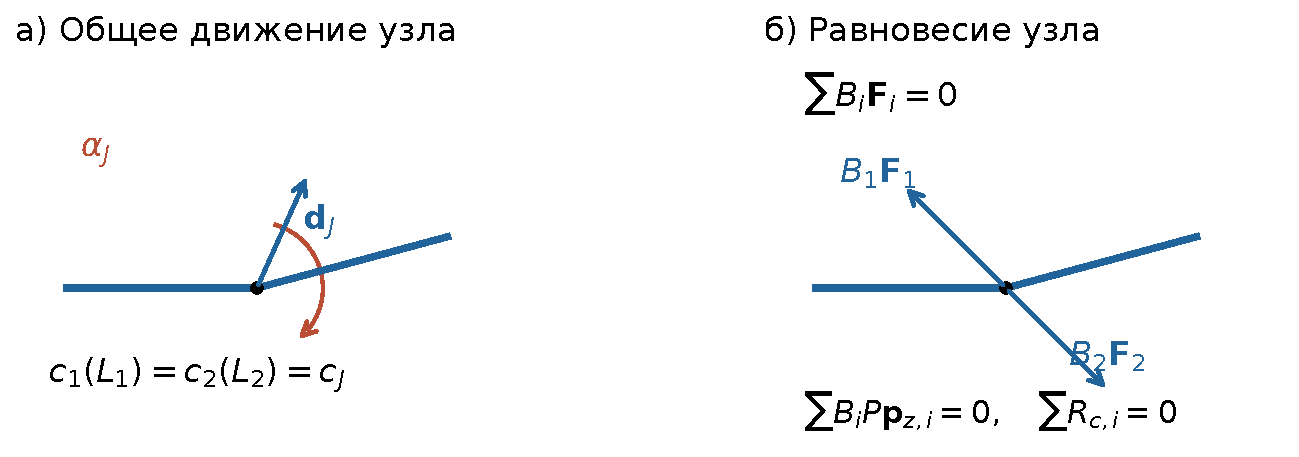
\includegraphics[width=\linewidth]{joint_compatibility_work.pdf}
\caption{Условная схема узлового сопряжения: а) общие перемещение $\mathbf d_J$, приращение поворота $\boldsymbol\alpha_J$ и скаляр $c_J$; б) равновесие глобальных сил и обобщённых моментов. Красная стрелка показывает плоскую компоненту положительного поворота вокруг $k=-E_Z$ (по часовой стрелке в виде $XY$). Направления сил условные, их реальные значения здесь не изображены. Узел не имеет самостоятельной массы или энергии.}
\label{fig:joint}
\end{figure}

\subsection{Баланс сил, моментов и усилий поля $c$}
Граничная виртуальная работа потенциальной энергии каждого плеча имеет вид
\[
[\mathbf F_i\cdot\delta\mathbf U_i+
\mathbf p_{z,i}\cdot\delta\mathbf z_i+R_{c,i}\delta c_i]_0^{L_i},
\]
где
\[
\mathbf F_i=\trunc{R_i\mathbf N_i},\qquad
\mathbf p_{z,i}=\trunc{P^TJ_r^T\mathbf M_i},\qquad
R_{c,i}=H_i c_{i,s}.
\]
$\mathbf F_i$ --- сила в исходных локальных направлениях. $\mathbf p_{z,i}$ --- обобщённый момент, сопряжённый именованным углам. Он не тождествен декартовому физическому моменту при конечном повороте.

При переходе к общим координатам используется
\[
T_{7,i}=\operatorname{diag}(B_i,B_iP,1),\qquad
q_{\rm global}=T_{7,i}q_{\rm local}.
\]
Эта матрица ортогональна. Сохранение виртуальной работы требует того же перехода для ковекторов усилий: $f_{\rm global}=T_{7,i}f_{\rm local}$. Силы нельзя преобразовывать по независимо выбранному правилу знаков.

Оба конца в узле имеют положительный граничный знак, поскольку $s_i=L_i$. Вариация по общим семи координатам~\eqref{eq:compat} даёт
\begin{equation}
\boxed{\sum_{i=1}^2 B_i\mathbf F_i=0,\qquad
\sum_{i=1}^2 B_iP\mathbf p_{z,i}=0,\qquad
\sum_{i=1}^2R_{c,i}=0.}
\label{eq:jointbalance}
\end{equation}
Первые три компоненты~\eqref{eq:jointbalance} --- баланс глобальных сил. Следующие три --- баланс обобщённых моментов; последнее условие --- баланс усилий независимой поперечной координаты. В неусечённой записи физический момент равен $BR\mathbf M$, где $\mathbf M=J_r^{-T}P\mathbf p_z$. В кубической модели и это преобразование выполняется согласованно по степени.

Таким образом, узел не добавляет собственной упругой или кинетической энергии. Общие скорости и балансы~\eqref{eq:jointbalance} обнуляют суммарную мощность внутренних узловых усилий. При неподвижных заделках и отсутствии внешних сил полная энергия принятой автономной модели сохраняется.

\section{Что именно решается численно}
\subsection{Последовательность шести задач}
\textbf{1. Пространственная дискретизация.} Семь полей каждого плеча представляются конечными суммами полиномиальных функций материальной координаты. Подстановка в вариационные уравнения и проекция на тот же допустимый базис дают систему Галёркина. Базис учитывает заделки и общий узел; все поля и физические коэффициенты сохраняются. Обозначения p12 и p14 означают уровни полиномиальной пространственной аппроксимации с параметрами $p=12$ и $p=14$ одной модели.

Дискретные коэффициенты полей соберём в $\mathbf q_h$. Кубические уравнения имеют форму
\[
\mathsf M(\mathbf q_h)\ddot{\mathbf q}_h+
\mathbf I(\mathbf q_h,\dot{\mathbf q}_h)+\nabla V_h(\mathbf q_h)=0.
\]
Здесь $\mathsf M$ --- переменная масса, $\mathbf I$ --- нелинейные инерционные члены. После обращения массы получаем автономную систему первого порядка $\dot X=f(X)$ для $X=(\mathbf q_h,\dot{\mathbf q}_h)$.

\textbf{2. Линейные собственные колебания.} В недеформированном состоянии решается задача $K_0\varphi=\omega^2M_0\varphi$. Формы содержат все необходимые поля и нормируются по массе. Номера 2 и 4 далее означают позиции в локальном упорядоченном плоском спектре фиксированной геометрии. Их физическая идентичность при увеличении $p$ проверена по профилям, а не назначена только по номеру.

\textbf{3. Свободное нелинейное периодическое движение.} Искомые плоские поля раскладываются по времени в ряд
\[
p_h(t)=p_{h,0}+\sum_{k=1}^{K_t}p_{h,k}\cos(k\Omega t),
\qquad p_h=(u_h,w_h,\theta_h,c_h).
\]
Метод гармонического баланса требует исчезновения временных проекций полной плоской кубической невязки. Неизвестны все коэффициенты и частота $\Omega$. Дополнительно задаётся физическая амплитуда $A=\max_{i,s}|w_i(s,0)|$. Она не заменяется первой модальной координатой. Косинусное представление соответствует обратимости по времени и нулевым скоростям выбранного начального состояния.

\textbf{4. Линеаризация около найденного движения.} Полный аналитический Jacobian $Df(X_0(t))$ вычисляется вдоль периодического плоского состояния. Зеркальная симметрия отделяет плоские и внеплоскостные возмущения. Переменная масса и нелинейная инерция остаются в обоих блоках.

\textbf{5. Спектральная устойчивость.} Периодические коэффициенты и возмущение раскладываются по временным гармоникам. Метод Хилла даёт характеристические показатели и множители Флоке. Проверяются пространственное и временное усечения, невязки собственного вектора и чувствительность к точности основного движения.

\textbf{6. Независимый динамический контроль.} Ранее найденное растущее направление воспроизведено прямой касательной динамикой и полной семиполевой нелинейной динамикой p12. Эти расчёты проверяют начальный рост малого возмущения на конечном интервале. Здесь они используются как сохранённые результаты; новые траектории не рассчитываются.

\subsection{Почему плоское основное движение содержит две формы}
Для выбранной геометрии сохранённые плоские частоты p12 равны
\[
\omega_{{\rm pl},2}=0.4348207304902722,\qquad
\omega_{{\rm pl},4}=1.3063293949106531.
\]
Их близость $\omega_{{\rm pl},4}\approx3\omega_{{\rm pl},2}$ создаёт внутренний резонанс 1:3. Кубическая нелинейность основной формы содержит третью временную гармонику; её проекция на четвёртую форму ненулевая. Деление на малый знаменатель $\omega_4^2-9\omega_2^2$ делает обычную одномодовую поправку большой и недостаточно контролируемой.

Поэтому обе формы входят в активное приближение:
\[
p\approx Q_2(t)\varphi_2+Q_4(t)\varphi_4+p_{\rm nr},
\qquad
Q_2\sim a_2\cos(\Omega t+\phi_2),\quad
Q_4\sim a_4\cos(3\Omega t+\phi_4).
\]
Каждая $\varphi_j$ включает четыре поля $u,w,\theta,c$. Амплитуда $a_4$ определяется вместе с основной частотой и формой, а не назначается из нерегулярной одномодовой поправки. $p_{\rm nr}$ содержит необходимые нерезонансные составляющие, среднюю конфигурацию и другие гармоники.

Построена ветвь с согласованной относительной фазой $\Psi=3\phi_2-\phi_4=0$, затем уточнённая в полном плоском пространстве. Она называется \emph{типом II}: начальное состояние специально подготовлено по периодическому решению и включает ненулевую четвёртую форму. \emph{Тип I} означает обычное начальное возбуждение преимущественно одной второй линейной формы. Эти начальные состояния различны; полученный результат устойчивости типа II не переносится автоматически на тип I.

На рис.~\ref{fig:modes} показаны рассчитанное плоское начальное положение и опасная пространственная форма. В подписях OUT означает внеплоскостное движение; OUT2 --- соответствие второй линейной внеплоскостной форме выбранной конструкции.
\begin{figure}[htbp]
\centering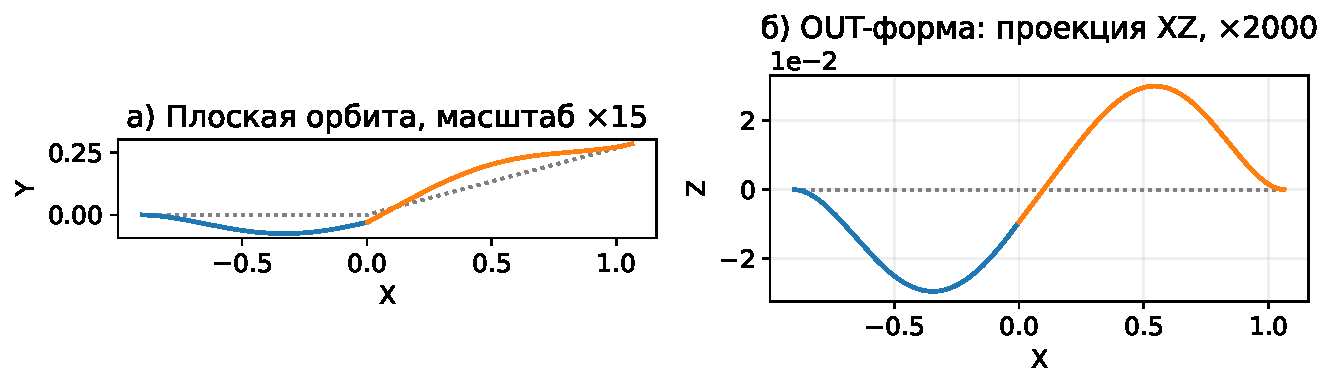
\includegraphics[width=\linewidth]{supervisor_physical_modes.pdf}
\caption{Сохранённые физические профили p14: слева --- плоское периодическое движение, перемещения увеличены в 15 раз; справа --- растущая внеплоскостная форма в проекции $XZ$. Справа её масштаб $\max(|v|,L_{\rm ref}|\Phi|,L_{\rm ref}|\psi|)$ приведён к $0.01A$ при $L_{\rm ref}=1$, затем перемещения увеличены в 2000 раз. Пунктир --- исходные оси; синее плечо --- первое, оранжевое --- второе. Масштабы $X$ и $Z$ справа различны. Это рассчитанные осевые профили, а не условные синусоиды; повороты сечений входят в расчёт, но не все видны на осевой линии.}
\label{fig:modes}
\end{figure}

\section{Как плоское движение может потерять внеплоскостную устойчивость}
\subsection{Инвариантность плоскости и линейная задача возмущений}
В идеально плоском начальном состоянии никакое внеплоскостное движение само по себе не появляется. Это следствие симметрии принятой модели. Однако инвариантная плоскость может быть неустойчивой: малое ненулевое отклонение способно увеличиваться.

Пусть $p_0(s,t)=(u_0,w_0,\theta_0,c_0)$ --- найденное плоское периодическое решение. Внесём малые пространственные поля, сохранив порядок семи координат:
\[
q(s,t)=(u_0,w_0,\varepsilon\eta_v,
\varepsilon\eta_\Phi,\varepsilon\eta_\psi,\theta_0,c_0).
\]
Параметр $\varepsilon$ характеризует малость возмущения независимо от конечной малой амплитуды основного движения. Сохраняем только линейные члены по $\eta_v,\eta_\Phi,\eta_\psi$ и их скоростям. После дискретизации получаем
\begin{equation}
\dot z_\perp=A_\perp[p_0(t)]z_\perp,
\qquad z_\perp=(\eta_\perp,\dot\eta_\perp),\quad
\eta_\perp=(\eta_v,\eta_\Phi,\eta_\psi).
\label{eq:tangent}
\end{equation}
Коэффициенты~\eqref{eq:tangent} периодически изменяются из-за движения $p_0$. Они содержат все гармоники, средние смещения, геометрические и инерционные связи. Использование одной постоянной упругой матрицы не воспроизводило бы эту задачу.

Близость $\Omega\approx2\omega_{\perp,2}$ выделяет параметрический канал 2:1. Плоское движение изменяет коэффициенты пространственного колебания с частотой около удвоенной собственной. Ненулевые смешанные члены принятой энергии обеспечивают связь положительной и отрицательной частотных ветвей. Частотная близость сама по себе ещё не гарантирует рост: необходимы соответствующие коэффициенты и полная согласованная спектральная проверка.

Внутренний резонанс 1:3 необходим для контролируемого описания выбранного плоского состояния. Но отдельная причинная необходимость именно четвёртой плоской формы для OUT-роста не установлена. Механизм 2:1 следует из принятой нелинейной модели, а не из непосредственно приложенной внеплоскостной силы.

\subsection{Показатели Флоке и метод Хилла}
Если период основного движения $T=2\pi/\Omega$, то $A_\perp(t+T)=A_\perp(t)$. Для периодической линейной системы решение имеет форму
\begin{equation}
z_\perp(t)=e^{\lambda t}p_F(t),\qquad p_F(t+T)=p_F(t),
\qquad \rho=e^{\lambda T}.
\label{eq:floquet}
\end{equation}
В~\eqref{eq:floquet} $p_F$ описывает изменение формы внутри периода. Множитель $\rho$ характеризует переход того же направления через целый период, а $\operatorname{Re}\lambda$ --- экспоненциальную огибающую. Условия $|\rho|>1$ и $\operatorname{Re}\lambda>0$ означают линейную неустойчивость конкретного периодического движения.

Раскладывая $A_\perp=\sum_m A_m e^{im\Omega t}$ и $p_F=\sum_n z_n e^{in\Omega t}$, из~\eqref{eq:tangent} получаем
\begin{equation}
\lambda z_n=\sum_m A_{n-m}z_m-in\Omega z_n.
\label{eq:hill}
\end{equation}
Знак последнего члена~\eqref{eq:hill} следует из дифференцирования Fourier-гармоники. Показатели, различающиеся на $ik\Omega$, задают один и тот же множитель и не являются разными физическими растущими режимами.

Для консервативной проверки скорости нельзя автоматически назвать каноническими импульсами. Импульс линейного возмущения имеет вид $\Pi=\mathsf M_\perp(t)\dot\eta+\mathsf C_\perp(t)\eta$. При переходе $Z=\mathsf S(t)z$ оператор преобразуется как
\[
\dot Z=(\dot{\mathsf S}\mathsf S^{-1}+\mathsf SA_\perp\mathsf S^{-1})Z.
\]
Член с $\dot{\mathsf S}$ необходим при переменной массе. Здесь $\mathsf S$ --- матрица перехода состояния, в отличие от сдвиговой жёсткости $S$. Каноническая структура, сопряжённые частотные ветви и обратный множитель проверялись с этим переходом.

Поскольку основное движение представлено приближённым гармоническим балансом, спектр относится к периодической вариационной системе около контролируемого приближения. Точность самой орбиты проверяется отдельно. Увеличение некоторой энергетической нормы за короткое время само по себе не устанавливает неустойчивость по Флоке.

\subsection{Рост малого возмущения и сохранение полной энергии}
Внеплоскостное возмущение растёт на фоне конечного основного движения. В полной автономной системе энергия может переходить от основного плоского колебания к пространственному движению; суммарная энергия сохраняется. Касательная система описывает начальную стадию, когда изменение основной орбиты из-за малого возмущения ещё несущественно. Отдельная энергия формы или вида движения не обязана сохраняться.

Если вещественный множитель отрицателен, растущее направление меняет знак за каждый период: $z(t+T)=\rho z(t)$ для соответствующего решения. При $\rho=-e^{\sigma T}$ модуль увеличивается, а знак чередуется. В комплексном представлении это соответствует мнимой части показателя $\Omega/2$ с точностью до Fourier-копий. Такая линейная смена знака не доказывает существование новой нелинейной орбиты периода $2T$.

Долговременный рост не может описываться касательной системой без ограничения: когда пространственная амплитуда становится существенной, меняется и основное движение. Нелинейное насыщение, большой выход из плоскости и влияние демпфирования требуют отдельного исследования и здесь не утверждаются.

\section{Обнаруженное неустойчивое движение}
Результаты получены для одной фиксированной конструкции:
\[
L_1=0.9,\quad L_2=1.1,\quad \beta=15^\circ,\quad
\mu=\frac{L_2-L_1}{L_1+L_2}=0.1,
\]
\[
b_1=b_2=0.05,\quad h_1=h_2=0.10,\quad
E=\rho=1,\quad \nu=0.3,\quad\kappa=5/6,\quad A=0.005.
\]
Числа $E=\rho=1$ определяют нормированную исследовательскую постановку, а не идентифицированный материал. Частоты и время относятся к её единицам; физическая единица секунды здесь не задана.

Пространственная дискретизация построена методом Галёркина с полиномиальными базисными функциями. Обозначения p12 и p14 означают два пространственных разрешения одной вариационной модели, с параметром степени $p=12$ и $p=14$. Внешние и узловые условия сохраняются при переходе между ними.

\subsection{Спектральное и динамическое подтверждение}
В p14 уточнённое движение содержит 108 плоских степеней свободы. Проверены представления с 11 и 13 временными гармониками, независимые фазовые невязки, постоянство энергии и положительность массы. Полная относительная невязка составляет около $9\cdot10^{-9}$; точность орбиты независимо проверена и достаточна для предусмотренных спектральных контролей. Переход p12$\to$p14 сохраняет фазовую ветвь и физические формы.

Основной результат спектральной проверки:
\begin{equation}
\begin{aligned}
\Omega_{14}&=0.435115458304,\qquad
\sigma_{\perp,14}=\operatorname{Re}\lambda=0.003411315508,\\
\rho_{\perp,14}&=-1.050493781532.
\end{aligned}
\label{eq:result}
\end{equation}
По~\eqref{eq:result} амплитуда растущей составляющей увеличивается примерно на $5.05\%$ за период и меняет знак. Характерное время увеличения в $e$ раз равно $t_e/T=20.3003$. Растущая форма преимущественно соответствует второй линейной внеплоскостной изгибно-крутильной форме (OUT2); в принятой квадратичной энергетической мере состава её изгибное участие равно $97.2997\%$. Кручение присутствует, поэтому форма не называется чисто изгибной.

\begin{center}\small
\begin{tabular}{lcc}
\hline
Величина & p12 & p14\\\hline
Частота плоской орбиты & 0.435115586723 & 0.435115458304\\
Показатель роста, метод Хилла & 0.003411410067 & 0.003411315508\\
Множитель Флоке & $-1.050495200663$ & $-1.050493781532$\\
Показатель, прямая касательная динамика & 0.003411405495 & ---\\
Полная нелинейная динамика, усиление $3T$ & 1.159262825 & ---\\
Полная нелинейная динамика, усиление $5T$ & 1.279292325 & ---\\\hline
\end{tabular}
\end{center}

Проверены временное и пространственное разрешения метода Хилла; итоговый p14 расчёт включает все 81 внеплоскостные моды. Разность показателей p12/p14 составляет $0.00277\%$; физические растущие состояния практически совпадают. Это сильное согласование двух разрешений, но не строгое доказательство полной пространственной сходимости.

В p12 рост воспроизведён прямым интегрированием касательной системы и полной нелинейной семиполевой динамикой. Начальное возмущение восстановлено из растущей формы Флоке и включает ненулевые скорости. Относительная ошибка согласования полной и касательной динамики до $5T$ равна $2.42\cdot10^{-6}$, а физический внеплоскостной прогиб остаётся менее $1\%$ амплитуды основного движения. Это динамическое подтверждение выбранного растущего направления, а не исследование произвольных начальных отклонений.

\begin{figure}[htbp]
\centering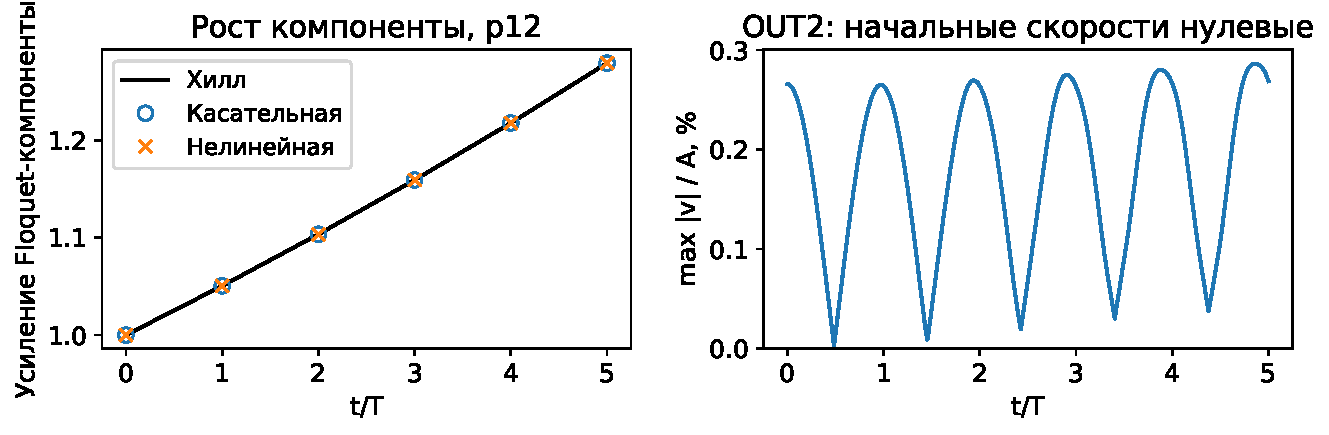
\includegraphics[width=\linewidth]{supervisor_growth_confirmation.pdf}
\caption{Слева --- рассчитанное ранее p12 усиление выбранной растущей составляющей: согласование спектрального прогноза Хилла, касательной и полной нелинейной динамики. Справа --- короткий p14 касательный контроль при отклонении по OUT2 с нулевыми скоростями: максимальный физический прогиб $\max|v|/A$. Левый и правый графики относятся к разным начальным возмущениям и разным наблюдаемым величинам; масштабы данных не увеличены.}
\label{fig:growth}
\end{figure}

\newpage
\subsection{Отклонить из плоскости и отпустить}
Более простое механическое начальное условие задаётся отклонением по линейной OUT2-форме, без начальных внеплоскостных скоростей. Сохранены все компоненты $v,\Phi,\psi$ и условия узла. Его масштаб равен
\[
\max_{i,s}\bigl(|v_i|,L_{\rm ref}|\Phi_i|,L_{\rm ref}|\psi_i|\bigr)
=5\cdot10^{-5},\qquad L_{\rm ref}=1.
\]
Корректная каноническая проекция с использованием двойственных мод на растущее подпространство ненулевая. Восстановленная растущая составляющая имеет $43.28\%$ полного начального физического масштаба и $48.96\%$ начального максимального прогиба. Эти числа не являются долями энергии: составляющие не ортогональны и могут взаимно компенсировать отдельные поля.

Один короткий касательный p14 контроль с такими начальными условиями, продолженный от $3T$ до $5T$, подтверждает усиление растущей составляющей до $1.159259$ и $1.279285$ соответственно. Общая норма возмущения по квадратичной энергии недеформированного состояния возрастает к $5T$ в $1.2180$ раза. При этом максимум физического прогиба за $3T$ равен $0.2753\%$ основной амплитуды, а за $5T$ --- $0.2864\%$; это показано справа на рис.~\ref{fig:growth}.

Таким образом, обычное начальное отклонение без скоростей способно возбуждать найденный механизм. На коротком интервале рост разрешим в модальной составляющей, но выход из плоскости физически мал. Мгновенный прогиб не обязан возрастать монотонно с тем же показателем. Спектральный прогноз только растущей составляющей даёт усиление $1.6366$ за $10T$ и $2.6784$ за $20T$; эти интервалы не интегрировались и большой пространственный прогиб ими не гарантируется.

\section{Область заключения и вопросы для обсуждения}
\textbf{Подтверждённое заключение.} В принятой нелинейной стержневой модели выявлена внеплоскостная неустойчивость конкретного свободного плоского периодического движения. Положительный показатель роста подтверждён спектральными и динамическими расчётами и сохраняется при увеличении пространственного разрешения с p12 до p14.

Плоская устойчивость имеет отдельное ограничение. У точной периодической орбиты автономной системы сдвиг времени создаёт нейтральное направление $\dot X_0$. Для приближённой орбиты гармонического баланса $r=\dot X_{\rm HB}-f(X_{\rm HB})$ справедливо
\[
\ddot X_{\rm HB}-Df(X_{\rm HB})\dot X_{\rm HB}=\dot r.
\]
Остаток p14 нейтральной проверки $7.59\cdot10^{-8}$ при допуске $2\cdot10^{-9}$ объяснён производной малой невязки гармонического баланса, преимущественно в 12-й гармонике. Jacobian и каноническое преобразование согласуются с этой тождественностью. В разрешённом ненейтральном плоском спектре роста не обнаружено, но полной устойчивости относительно всех плоских возмущений не установлено. Это не отменяет отдельный подтверждённый внеплоскостной результат.

Результат относится к одной геометрии, одной амплитуде и специально подготовленной ветви типа II. Аналогичная неустойчивость для типа I не проверена. Длительное нелинейное насыщение и демпфирование не исследовались. Физическая применимость нелинейного закона, идеального узла и условия $c_1=c_2$ остаётся допущением. Независимые трёхмерная FEM и экспериментальная проверка отсутствуют. Граница применимости плоской модели пока не определена.

\subsection*{Вопросы для научного руководителя}
\begin{enumerate}
\setlength{\itemsep}{1pt}
\item Насколько физически оправданы принятая нелинейная редукция и идеальное угловое сопряжение, включая общую поперечную координату $c$?
\item Следует ли сначала проверить линейный спектр независимой трёхмерной FEM?
\item Нужно ли исследовать возбуждение найденного механизма при обычных начальных условиях типа I?
\item Когда следует вводить демпфирование для оценки наблюдаемости роста?
\item Что целесообразнее сделать основным конечным результатом диссертации: конкретный механизм параметрической неустойчивости или область практической применимости плоской модели?
\end{enumerate}

\subsection*{Использованные источники}
Литературные основания редуцированных линейных блоков отделены выше от принятого нелинейного продолжения и полученных численных результатов. Исходная работа Миндлина --- Геррманна изложена по~\cite{jang,rucka}; её полный текст непосредственно не использовался.

{\raggedright
\begin{thebibliography}{4}
\bibitem{jang} Jang I., Park I., Lee U. Guided waves in a Timoshenko beam with a bonded composite patch: Frequency domain spectral element modeling and analysis // Composites Part B: Engineering. 2014. Vol. 60. P. 248--260. DOI: 10.1016/j.compositesb.2013.12.050.
\bibitem{rucka} Rucka M. Experimental and numerical study on damage detection in an L-joint using guided wave propagation // Journal of Sound and Vibration. 2010. Vol. 329, No. 10. P. 1760--1779. DOI: 10.1016/j.jsv.2009.12.004.
\bibitem{crespo} Crespo da Silva M. R. M. Non-linear flexural-flexural-torsional-extensional dynamics of beams---I. Formulation // International Journal of Solids and Structures. 1988. Vol. 24, No. 12. P. 1225--1234. DOI: 10.1016/0020-7683(88)90087-X.
\bibitem{yartsev} Ярцев Б. А. Связанные колебания композитных конструкций. СПб.: ФГУП «Крыловский государственный научный центр», 2024. 216 с. ISBN 978-5-6048511-4-2.
\end{thebibliography}
}

\appendix
\section{Скалярные ряды для восстановления семи кубических уравнений}
Ниже заданы все необходимые компоненты кинематических операторов.
Подстановка рядов в~\eqref{eq:cubictrans},~\eqref{eq:cubicrot} с последующим усечением однозначно восстанавливает каждое уравнение. Это компактное раскрытие сохранённого полиномиального вывода, без новых физических членов.

Положим $a^2=\Phi^2+\psi^2+\theta^2$. Компоненты матрицы $R$ до третьей степени равны
\[
\begin{array}{lll}
R_{11}=1-\tfrac12(\psi^2+\theta^2),&
R_{12}=-\theta-\tfrac12\Phi\psi+\tfrac16a^2\theta,&
R_{13}=-\psi+\tfrac12\Phi\theta+\tfrac16a^2\psi,\\[4pt]
R_{21}=\theta-\tfrac12\Phi\psi-\tfrac16a^2\theta,&
R_{22}=1-\tfrac12(\Phi^2+\theta^2),&
R_{23}=-\Phi-\tfrac12\psi\theta+\tfrac16a^2\Phi,\\[4pt]
R_{31}=\psi+\tfrac12\Phi\theta-\tfrac16a^2\psi,&
R_{32}=\Phi-\tfrac12\psi\theta-\tfrac16a^2\Phi,&
R_{33}=1-\tfrac12(\Phi^2+\psi^2).
\end{array}
\]
В произведениях с силами первой степени компоненты $R$ нужны лишь до второй степени, но здесь приведён полный третий порядок для проверки геометрии.

Все три деформации до степени 3 записываются как
\[
\begin{aligned}
\relax[\Gamma_1]_{\leq3}={}&u_s+\theta w_s+\psi v_s-\tfrac12(\theta^2+\psi^2)\\
&-\tfrac12u_s(\theta^2+\psi^2)-\tfrac12\Phi\psi w_s+\tfrac12\Phi\theta v_s,\\
[\Gamma_2]_{\leq3}={}&w_s-\theta-\theta u_s+\Phi v_s-\tfrac12\Phi\psi\\
&+\tfrac16a^2\theta-\tfrac12\Phi\psi u_s
-\tfrac12(\Phi^2+\theta^2)w_s-\tfrac12\psi\theta v_s,\\
[\Gamma_3]_{\leq3}={}&v_s-\psi-\psi u_s-\Phi w_s+\tfrac12\Phi\theta\\
&+\tfrac16a^2\psi+\tfrac12\Phi\theta u_s
-\tfrac12\psi\theta w_s-\tfrac12(\Phi^2+\psi^2)v_s.
\end{aligned}
\]
Они согласуются с линейными сдвигами и квадратичными компонентами~\eqref{eq:Gamma2}. При $\Phi=\psi=v=0$ получаются два ряда плоской системы.

Для $d=s$ или $d=t$ введём $D_d=\Phi\Phi_d+\psi\psi_d+\theta\theta_d$. Обозначим компоненты через $h_{d,i}$:
\[
\begin{aligned}
h_{d,1}&=\Phi_d+\tfrac12(\psi\theta_d-\theta\psi_d)
+\tfrac16(\Phi D_d-a^2\Phi_d),\\
h_{d,2}&=-\psi_d+\tfrac12(\Phi\theta_d-\theta\Phi_d)
+\tfrac16(-\psi D_d+a^2\psi_d),\\
h_{d,3}&=\theta_d+\tfrac12(\Phi\psi_d-\psi\Phi_d)
+\tfrac16(\theta D_d-a^2\theta_d).
\end{aligned}
\]
При $d=s$ эти величины равны $[\chi_i]_{\leq3}$, при $d=t$ --- $[\Omega_i]_{\leq3}$. Указанные ряды, силы и моменты из основного текста задают всю кубическую систему, включая смешанные ускорения и переменную массу. Огромный одночленный перечень для использования отчёта не требуется.

В пространственных балансах $N_i,M_i,\ell_i$ следует сначала составить произведения до необходимой степени, выполнить пространственные и временные производные, затем координатное преобразование. Производные сохраняют амплитудную степень. Равенство такого построения координатным уравнениям действия проверено ранее двумя независимыми полиномиальными путями для всех $7\times3$ однородных частей.

\section{Однозначное полиномиальное действие до четвёртой степени}
Приложение раскрывает коэффициенты действия~\eqref{eq:quartic} и тем самым полностью определяет операторы системы~\eqref{eq:cubictrans},~\eqref{eq:cubicrot}. Оно является компактной записью уже принятого разложения.

Положим $\Gam=\boldsymbol\gamma_1+\boldsymbol\gamma_2+\boldsymbol\gamma_3+O(\varepsilon_a^4)$, где
\[
\begin{aligned}
\boldsymbol\gamma_1&=\mathbf U_s-\mathbf a\times\eone,\\
\boldsymbol\gamma_2&=-\mathbf a\times\mathbf U_s+\tfrac12\mathbf a\times(\mathbf a\times\eone),\\
\boldsymbol\gamma_3&=\tfrac12\mathbf a\times(\mathbf a\times\mathbf U_s)
-\tfrac16\mathbf a\times[\mathbf a\times(\mathbf a\times\eone)].
\end{aligned}
\]
Для $d=s,t$ определим $\mathbf h_{d,1}=\mathbf a_d$, $\mathbf h_{d,2}=-\mathbf a\times\mathbf a_d/2$, $\mathbf h_{d,3}=\mathbf a\times(\mathbf a\times\mathbf a_d)/6$. При $d=s$ это $\Chi_1,\Chi_2,\Chi_3$; при $d=t$ --- $\Om_1,\Om_2,\Om_3$. Второй индекс в $\gamma_{n,1}$ далее означает первую компоненту вектора $\boldsymbol\gamma_n$. Матрицы инерции по степеням равны
\[
\begin{aligned}
J_0&=\operatorname{diag}(j_\perp+j_\parallel,j_\perp,j_\parallel),\\
J_1&=2c\operatorname{diag}(j_\parallel,0,j_\parallel),\qquad
J_2=c^2\operatorname{diag}(j_\parallel,0,j_\parallel).
\end{aligned}
\]
Тогда
\[
\begin{aligned}
T_2&=\tfrac m2|\mathbf U_t|^2+\tfrac{j_\parallel}{2}c_t^2+\tfrac12\Om_1^TJ_0\Om_1,\\
T_3&=\Om_1^TJ_0\Om_2+\tfrac12\Om_1^TJ_1\Om_1,\\
T_4&=\tfrac12\Om_2^TJ_0\Om_2+\Om_1^TJ_0\Om_3
+\Om_1^TJ_1\Om_2+\tfrac12\Om_1^TJ_2\Om_1,\\[2pt]
V_2&=\tfrac12\boldsymbol\gamma_1^TD_\Gamma\boldsymbol\gamma_1
+\nu Cc\gamma_{1,1}+\tfrac C2c^2+\tfrac H2c_s^2+\tfrac12\Chi_1^TD_\chi\Chi_1,\\
V_3&=\boldsymbol\gamma_1^TD_\Gamma\boldsymbol\gamma_2+\nu Cc\gamma_{2,1}
+\Chi_1^TD_\chi\Chi_2,\\
V_4&=\tfrac12\boldsymbol\gamma_2^TD_\Gamma\boldsymbol\gamma_2
+\boldsymbol\gamma_1^TD_\Gamma\boldsymbol\gamma_3+\nu Cc\gamma_{3,1}
+\tfrac12\Chi_2^TD_\chi\Chi_2+\Chi_1^TD_\chi\Chi_3.
\end{aligned}
\]
Материальные коэффициенты имеют нулевую амплитудную степень. Пространственные и временные производные сохраняют степень поля. Дифференцирование этого $L_{\leq4}$ по каждому из семи полей даёт ровно однородные остатки уравнений степеней 1, 2 и 3.

\subsection*{Крутильный коэффициент прямоугольника}
В текущем изотропном пределе обобщённой редукции~\cite{yartsev} связь кручения с анизотропными упругими компонентами равна нулю. Для принятого соответствия размеров исходная прямоугольная формула имеет вид
\begin{equation}
C_T=\frac{G b^3h}{3}\left[1-\frac{192b}{\pi^5h}
\sum_{r=0}^{\infty}\frac{\tanh\!\left((2r+1)\pi h/(2b)\right)}{(2r+1)^5}\right].
\label{eq:CT}
\end{equation}
Она относится к действующим ориентациям сечения и не заменяет крутильную жёсткость полярным моментом. В расчётах использован уже проверенный коэффициент этой модели; заново он при подготовке отчёта не вычислялся.
\end{document}
